% Short Cambridge SRG seminar: 26 frames in seven acts, no overlays or appendix.
% Same preamble as talk.tex; frames live in short/. Spoken notes and hidden Q&A
% detail generate PRESENTER-GUIDE-SHORT.md via tools/presenter_guide.py --short.
\documentclass[aspectratio=169,10pt]{beamer}
% Packages, TikZ libraries and Beamer options.
\usepackage[T1]{fontenc}
\usepackage[utf8]{inputenc}
\usepackage{lmodern,amsmath,amssymb,mathtools,booktabs,array,tabularx,tikz}
\usepackage{appendixnumberbeamer}
\usepackage{listings}
\lstdefinestyle{slidepython}{language=Python,basicstyle=\ttfamily\fontsize{10.5}{14}\selectfont,keywordstyle=\color{Teal}\bfseries,commentstyle=\color{Muted},stringstyle=\color{Gold},showstringspaces=false,columns=fullflexible,keepspaces=true,aboveskip=4pt,belowskip=4pt,xleftmargin=0pt,breaklines=false}
\usetikzlibrary{arrows.meta,positioning,calc,fit,backgrounds}
\usefonttheme{professionalfonts}
\setbeameroption{hide notes}

% Colours and Beamer theme settings.
\definecolor{Ink}{HTML}{142B3B}
\definecolor{Teal}{HTML}{007E87}
\definecolor{Gold}{HTML}{AD701B}
\definecolor{Rust}{HTML}{B34233}
\definecolor{Muted}{HTML}{536874}
\definecolor{Pale}{HTML}{EFF5F5}
\definecolor{Sand}{HTML}{FBF3E6}
\definecolor{Line}{HTML}{C9D6DB}
\setbeamercolor{normal text}{fg=Ink,bg=white}
\setbeamercolor{structure}{fg=Teal}
\setbeamercolor{frametitle}{fg=Ink,bg=white}
\setbeamercolor{alerted text}{fg=Rust}
\setbeamerfont{frametitle}{size=\fontsize{19}{22}\selectfont,series=\bfseries}
\setbeamersize{text margin left=.8cm,text margin right=.8cm}
\setbeamertemplate{navigation symbols}{}
\setbeamertemplate{itemize item}{\color{Teal}\scriptsize$\bullet$}
\setbeamertemplate{itemize subitem}{\color{Muted}\scriptsize$\circ$}
\setbeamertemplate{enumerate item}{\color{Teal}\bfseries\insertenumlabel.}

% Frame-title strip, evidence tags, text and table helpers, the fork-tree symbol.
% Section strip on every frame: the current section shows its number and name in teal, the others their number.
\newcommand{\currentact}{0}
\newcommand{\setact}[1]{\renewcommand{\currentact}{#1}}
\newcommand{\actitem}[2]{\ifnum\currentact=#1{\color{Teal}\bfseries #1\enspace #2}\else{\color{Muted!65}#1}\fi}
% Evidence tag: \ev{\tagM} inside a frame title prints the tag on the part-label line.
\newcommand{\currentev}{}
\newcommand{\currentsurf}{}
\newcommand{\surf}[1]{\gdef\currentsurf{#1}}
\newcommand{\ev}[1]{\gdef\currentev{#1}}
\newcommand{\evtag}[2]{\tikz[baseline=(x.base)]\node[draw=#1,text=#1,line width=.6pt,rounded corners=1.5pt,inner xsep=2.4pt,inner ysep=1.3pt,font=\fontsize{7.6}{8.4}\selectfont\bfseries](x){#2};}
\newcommand{\tagM}{\evtag{Teal}{MEASURED}}
\newcommand{\tagB}{\evtag{Ink}{BUILT}}
\newcommand{\tagP}{\evtag{Gold}{PROPOSED}}
\newcommand{\tagO}{\evtag{Muted}{PUBLISHED}}
\newcommand{\tagA}{\evtag{Gold!55!Muted}{ANALOGY}}
\newif\ifbackup
\def\endlabel{REFERENCES}\newcommand{\setendlabel}[1]{\gdef\endlabel{#1}}
\newcommand{\actstrip}{\ifbackup{\color{Teal}\bfseries\endlabel}\else\actitem{1}{INTRODUCTION}\quad\actitem{2}{CASE STUDY}\quad\actitem{3}{DESIGN}\quad\actitem{4}{ANALYSIS}\quad\actitem{5}{EVALUATION}\quad\actitem{6}{CONCLUSION}\fi}
\setbeamertemplate{frametitle}{\gdef\currentev{}\gdef\currentsurf{}\sbox0{\insertframetitle}\vspace{.1cm}{\fontsize{8}{9.5}\selectfont\actstrip\ifx\currentsurf\empty\else\quad{\color{Gold}\bfseries\MakeUppercase{\currentsurf}}\fi\hfill\currentev\par}\vspace{.08cm}\insertframetitle\par\vspace{.15cm}}
\setbeamertemplate{footline}{\hspace{.8cm}{\fontsize{7}{8}\selectfont\color{Muted}Yossi Eliaz\quad Cambridge SRG\quad 15 October 2026}\hfill{\fontsize{8}{9}\selectfont\color{Muted}\ifbackup\else\insertframenumber\,/\,\inserttotalframenumber\fi}\hspace{.8cm}\vspace{.17cm}}
\setlength{\tabcolsep}{5pt}
\renewcommand{\arraystretch}{1.15}
\newcolumntype{Y}{>{\raggedright\arraybackslash}X}
\newcolumntype{L}[1]{>{\raggedright\arraybackslash}p{#1}}
\newcommand{\lead}[1]{{\fontsize{12.5}{15}\selectfont #1\par}\vspace{.2cm}}
\newcommand{\claim}[1]{\par\vspace{.2cm}{\fontsize{11.5}{14}\selectfont\color{Teal}\bfseries #1\par}}
\newcommand{\sources}[1]{\par\vfill{\fontsize{7.8}{9.2}\selectfont\color{Muted}#1\par}\vspace{.05cm}}
\newcommand{\tagline}[1]{\par{\fontsize{9}{11}\selectfont\color{Muted}#1\par}}
\newcommand{\term}[1]{\textbf{#1}}
\newcommand{\no}{{\color{Rust}\bfseries$\times$}}
\newenvironment{ticks}{\setlength{\leftmargini}{1.3em}\begin{itemize}\setlength{\itemsep}{1.5pt}}{\end{itemize}}
\newcommand{\yes}{{\color{Teal}\bfseries$\checkmark$}}
% Recurring symbol: the title slide's fork tree, inline beside the refrain (slides 10, 36, 50).
\newcommand{\forktree}[1][Teal]{\tikz[baseline={(0,-.55ex)},x=1em,y=1em]{\draw[#1,line width=.75pt] (0,0)--(.85,0)--(1.55,.42) (.85,0)--(1.55,0) (.85,0)--(1.55,-.42);\foreach \fx/\fy in {0/0,.85/0,1.55/.42,1.55/0,1.55/-.42}{\fill[#1] (\fx,\fy) circle(.12);}}}

% Secondary details are retained in source and extracted into the presenter guide.
\newcommand{\qadetail}[1]{}
% Recurring proposed continuation lifecycle; focus: 1 state, 2 evidence, 3 authority, 0 all.
\newcommand{\lifecycle}[1]{%
\def\ls{Ink!35}\def\le{Ink!35}\def\la{Ink!35}%
\ifnum#1=0\relax\def\ls{Teal}\def\le{Teal}\def\la{Teal}\fi%
\ifnum#1=1\relax\def\ls{Teal}\fi%
\ifnum#1=2\relax\def\le{Teal}\fi%
\ifnum#1=3\relax\def\la{Teal}\fi%
\begin{center}
\begin{tikzpicture}[x=1cm,y=1cm, every node/.style={align=center,font=\fontsize{9.5}{11}\selectfont}, lc/.style={draw=Ink!35,fill=Pale,text width=3.15cm,minimum height=.72cm,inner sep=3pt}, active/.style={draw=Teal,line width=1pt}]
\node[lc,draw=\ls] (a) at (0,0) {Identify useful state};
\node[lc,draw=\ls] (b) at (4,0) {Create continuations};
\node[lc,draw=\le] (c) at (8,0) {Return artifact + observations};
\node[lc,draw=\le] (d) at (8,-1.15) {Select or compose};
\node[lc,draw=\le] (e) at (4,-1.15) {Verify exact\\artifact};
\node[lc,draw=\la] (f) at (0,-1.15) {Controller\\authorizes\\publication};
\draw[flow] (a)--(b);\draw[flow] (b)--(c);\draw[flow] (c)--(d);\draw[flow] (d)--(e);\draw[flow] (e)--(f);
\end{tikzpicture}
\end{center}}

% Shared TikZ node and arrow styles.
\tikzset{state/.style={draw=Ink,line width=.9pt,fill=Pale,minimum height=.8cm,align=center,font=\small}, candidate/.style={draw=Gold,line width=.9pt,fill=Sand,minimum height=.8cm,align=center,font=\small}, evidence/.style={draw=Teal,line width=.9pt,fill=Pale,minimum height=.8cm,align=center,font=\small}, bad/.style={draw=Rust,line width=.9pt,fill=white,minimum height=.8cm,align=center,font=\small}, missing/.style={draw=Rust,dashed,line width=.9pt,fill=white,minimum height=.8cm,align=center,font=\small,text=Rust}, flow/.style={-{Latex[length=2mm]},draw=Ink,line width=.9pt}, message/.style={-{Latex[length=2mm]},draw=Teal,dashed,line width=.9pt}, denied/.style={-{Latex[length=2mm]},draw=Rust,line width=.9pt}, relation/.style={draw=Rust,densely dotted,line width=1.3pt}, labeltext/.style={font=\footnotesize,text=Muted,align=center}, proposed/.style={draw=Gold,dashed,line width=.9pt,fill=white,minimum height=.8cm,align=center,font=\small}}

% Title, author, PDF metadata and spacing.
\title{Forkable Sandboxes}
\subtitle{Reusable execution for self-driving computers}
\author{Yossi Eliaz}
\institute{Principal Engineer, Incredibuild; Senior Lecturer, HIT}
\date{Cambridge SRG, 15 October 2026}
\hypersetup{pdftitle={Forkable Sandboxes: Reusable Execution for Self-Driving Computers},pdfauthor={Yossi Eliaz},pdfsubject={From biological physics and genomics to adaptive execution: reusable state, evidence and authority},colorlinks=true,urlcolor=Teal,linkcolor=Ink}
\AtBeginDocument{\setlength{\abovedisplayskip}{6pt}\setlength{\belowdisplayskip}{6pt}\setlength{\abovedisplayshortskip}{3pt}\setlength{\belowdisplayshortskip}{3pt}}
\renewenvironment{center}{\par\vspace{.10cm}\centering}{\par\vspace{.10cm}}

% Short-deck overrides, loaded after the shared preamble.
% Landmarks: every footer shows the six sections with the current one in teal;
% Open questions get their own act (6) so the conclusion is one slide (7).
\renewcommand{\actstrip}{{\color{Teal}\bfseries\currentact\enspace\ifcase\currentact\or MOTIVATION\or EXAMPLES\or RUNTIME\or EVIDENCE\or ACCEPTANCE\or OPEN QUESTIONS\or CONCLUSION\fi}}
% acts 3-5 put their rule in the gold \surf label: COMPUTE ONCE, COUNT ONCE, PUBLISH ONCE.
% Rule chip (gold, filled) for claim lines on slides 10-14 (their \providecommand copies are no-ops);
% slide 5 draws the same chip with \colorbox because it sits inside a TikZ node.
\newcommand{\exchip}[1]{\tikz[baseline=(x.base)]\node[fill=Gold,text=white,rounded corners=1.5pt,inner xsep=2.6pt,inner ysep=1.7pt,font=\fontsize{7.6}{8.6}\selectfont\bfseries](x){#1};}
\newcommand{\progitem}[2]{\ifnum\currentact=#1{\color{Teal}\bfseries #2}\else{\color{Muted!55}#2}\fi}
\setbeamertemplate{footline}{\hspace{.8cm}{\fontsize{7}{8}\selectfont\color{Muted}Yossi Eliaz\quad Cambridge SRG}\hfill{\fontsize{7}{8}\selectfont\progitem{1}{Motivation}\enspace\progitem{2}{Examples}\enspace\progitem{3}{Runtime}\enspace\progitem{4}{Evidence}\enspace\progitem{5}{Acceptance}\enspace\progitem{6}{Open questions}\enspace\progitem{7}{Conclusion}}\hfill{\fontsize{8}{9}\selectfont\color{Muted}\insertframenumber\,/\,\inserttotalframenumber}\hspace{.8cm}\vspace{.17cm}}

\begin{document}
\setact{1}
% Title: the thesis, the arc and the refrain. The fork tree returns on the three MAP slides (rules, synthesis, contributions).
\begin{frame}[t]{Forkable sandboxes let computers explore alternatives without doing work twice.}
\vspace{0pt}
{\fontsize{17}{21}\selectfont\color{Teal}Self-organization $\to$ self-driving cars\par $\to$ self-driving compute.\par}
\vspace{.22cm}
{\fontsize{17}{20}\selectfont\forktree\quad\textbf{Compute once. Count once. Publish once.}\par}
\vspace{.22cm}
{\fontsize{12.5}{15}\selectfont\textbf{Yossi Eliaz}\par{\color{Muted}Principal Engineer, Incredibuild\par Associate Professor, HIT\par}}
\sources{Cambridge Systems Research Group, 15 October 2026. Employer affiliation disclosed.\\Tags:\enspace\tagO\ published work\quad\tagM\ our measurements\quad\tagB\ our code\\\phantom{Tags:}\enspace\tagP\ proposed, not run\quad\tagA\ worked example}
\qadetail{The integrated architecture is a research design. Individual implementations, published examples and own measurements are labeled on their respective slides. Employer affiliation does not imply endorsement. The fork-tree symbol stands for the proposed loop: reuse a reached state, run private alternatives, return evidence, and let one controller outside the child accept one checked result. The refrain names the three obligations that sharing work creates: compute once (runtime), count once (evidence), publish once (acceptance). Our own factory runs were serial on Docker sandboxes; nothing forked. A motivating future workload is a running application at a reproduced failure, with relevant process memory and local state; it has not been exercised in the factory case study. Select a worktree, warm image, disk snapshot, or verified process or VM checkpoint according to the state the next step reads. Disclosure and affiliations match the supplied Cambridge deck.}
\note{[0:35] My path runs from self-organization in cells, to self-driving cars, to self-driving compute. Say we have paid to reach a useful state. Can we try several next steps from there without paying for it again? My answer has three rules. Compute once. Count once. Publish once. The corner tags mark what is published, measured, built or only designed. First, where these ideas come from.}
\end{frame}

% Act 1: the waste. Two timing panels on one time scale, then the three old tools that remove it.
\begin{frame}[t]{\ev{\tagA}In parallel computing, the costly work is the work done twice.}
\vspace{.05cm}
\noindent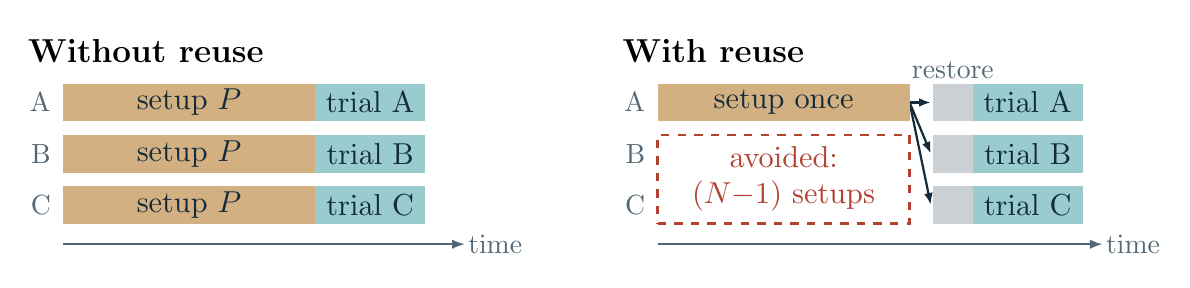
\begin{tikzpicture}[x=1cm,y=1cm,
  ph/.style={anchor=west,inner sep=0pt,font=\fontsize{12.5}{15}\selectfont\bfseries},
  rl/.style={anchor=east,inner sep=0pt,font=\fontsize{10}{12}\selectfont,text=Muted},
  bl/.style={font=\fontsize{11}{13}\selectfont,text=Ink}]
\useasboundingbox (0,.65) rectangle (14.4,-2.3);
% Without reuse: every trial repeats the setup.
\node[ph] at (0,.35) {Without reuse};
\foreach \rr/\yy in {A/-.3,B/-.95,C/-1.6}{
  \node[rl] at (.3,\yy) {\rr};
  \fill[Gold!55] (.45,\yy-.24) rectangle (3.65,\yy+.24);
  \node[bl] at (2.05,\yy) {setup $P$};
  \fill[Teal!40] (3.65,\yy-.24) rectangle (5.05,\yy+.24);
  \node[bl] at (4.35,\yy) {trial \rr};}
\draw[-{Latex[length=1.6mm]},Muted,line width=.6pt] (.45,-2.1)--(5.55,-2.1) node[right,labeltext,inner sep=1pt,font=\fontsize{10}{12}\selectfont] {time};
% With reuse: one setup, then every trial restores the saved state.
\begin{scope}[xshift=7.55cm]
\node[ph] at (0,.35) {With reuse};
\foreach \rr/\yy in {A/-.3,B/-.95,C/-1.6}{
  \node[rl] at (.3,\yy) {\rr};
  \fill[Ink!22] (3.95,\yy-.24) rectangle (4.45,\yy+.24);
  \fill[Teal!40] (4.45,\yy-.24) rectangle (5.85,\yy+.24);
  \node[bl] at (5.15,\yy) {trial \rr};
  \draw[Ink,line width=.8pt,-{Latex[length=1.5mm]}] (3.65,-.3)--(3.92,\yy);}
\fill[Gold!55] (.45,-.54) rectangle (3.65,-.06);
\node[bl] at (2.05,-.3) {setup once};
\node[labeltext,anchor=south,inner sep=1pt,font=\fontsize{10}{12}\selectfont] at (4.2,-.04) {restore};
\node[missing,inner sep=0pt,minimum width=3.2cm,minimum height=1.13cm,font=\fontsize{11}{13}\selectfont] at (2.05,-1.275) {avoided:\\$(N{-}1)$ setups};
\draw[-{Latex[length=1.6mm]},Muted,line width=.6pt] (.45,-2.1)--(6.1,-2.1) node[right,labeltext,inner sep=1pt,font=\fontsize{10}{12}\selectfont] {time};
\end{scope}
\end{tikzpicture}
\par\vspace{.25cm}
{\fontsize{13}{16}\selectfont
\begin{tabular}{@{}l@{\quad}l@{}}
{\color{Teal}\bfseries Cache} & reuse a previous run's output.\\
{\color{Teal}\bfseries Fork} & reuse a reached state.\\
{\color{Teal}\bfseries Sandbox} & keep each trial's writes private.\\
\end{tabular}\par}
\sources{Schematic, one time scale in both panels. Restoring is not free; the runtime section prices it.}
\qadetail{Illustrative task structure, not a measurement: bar lengths are schematic and use one time scale in both panels. The picture counts total work, not elapsed time; with three machines the right panel finishes slightly later, because each child restores, but it pays for one setup instead of three. Restoring is not free: saving the state once (H), restoring each child (R) and keeping each child's changes private (D) all cost, and the runtime section prices them against a warm cache, which is itself reuse. The avoided work is N-1 setups only when the restored state is what the next step reads; a cached file template may be an adequate and cheaper baseline. No timing or correctness result is attributed to these three trials. Our own factory runs were serial; nothing forked. Caches, forks and sandboxes are established mechanisms; slide 9 lists known systems.}
\note{[1:00] A question for you. How much of your last CI run was work another machine had already done? Often it is the same install and the same compile, again. On the left, three trials each repeat the same setup. On the right, we set up once, save that state, and start every trial from it. The gold blocks we skip are the waste: N minus one setups. Three old tools remove it. A cache reuses a previous run's output. A fork reuses a reached state. A sandbox keeps each trial's writes private, so sharing is safe. In a parallel, distributed world, the expensive thing is doing work twice. But sharing work creates obligations.}
\end{frame}

% THE MAP. One three-column geometry, drawn by \rulemap, appears on slides 3, 15 and 26.
% The same \providecommand block opens 03, 15 and 26; the first one loaded defines it, so all three
% slides draw identical headers, arrows, sub-headers and body anchors. Edit all three together.
% Arguments: #1 #2 #3 = column bodies (compute once, count once, publish once); #4 = extra TikZ.
\providecommand{\rulemap}[4]{%
\noindent\begin{tikzpicture}[x=1cm,y=1cm,
  rh/.style={evidence,text width=4.2cm,minimum height=.9cm,font=\fontsize{12}{14}\selectfont\bfseries,text=Teal},
  rs/.style={anchor=north,inner sep=0pt,font=\fontsize{10}{12}\selectfont,text=Muted},
  rb/.style={anchor=north,inner sep=0pt,text width=4.7cm,align=center,font=\fontsize{12}{14.5}\selectfont}]
\useasboundingbox (0,1.05) rectangle (14.4,-3.75);
\node[rh] (r1) at (2.3,0) {1\enspace COMPUTE ONCE};
\node[rh] (r2) at (7.2,0) {2\enspace COUNT ONCE};
\node[rh] (r3) at (12.1,0) {3\enspace PUBLISH ONCE};
\draw[flow] (r1)--(r2);\draw[flow] (r2)--(r3);
\draw[message] (r3.north)--++(0,.42)-|node[pos=.25,above,inner sep=1.5pt,font=\fontsize{9}{10}\selectfont,text=Teal]{continue} (r1.north);
\node[rs] at (2.3,-.62) {Runtime};
\node[rs] at (7.2,-.62) {Evidence};
\node[rs] at (12.1,-.62) {Acceptance};
\node[rb] at (2.3,-1.15) {#1};
\node[rb] at (7.2,-1.15) {#2};
\node[rb] at (12.1,-1.15) {#3};
#4
\end{tikzpicture}\par}
\begin{frame}[t]{\ev{\tagP}\surf{THREE RULES}Sharing work creates three rules.}
\vspace{.1cm}
\rulemap{When does reusing a state beat rebuilding it?}
{What must each parallel trial return?}
{Which exact bytes may we publish, and who decides?}
{\foreach \xx/\lab in {2.3/a cost rule,7.2/an evidence contract,12.1/an acceptance gate}{\draw[flow,draw=Teal] (\xx,-2.3)--(\xx,-2.68);\node[anchor=north,inner sep=0pt,font=\fontsize{12}{14.5}\selectfont\bfseries,text=Teal] at (\xx,-2.8) {\lab};}}
\claim{\centering\forktree\enspace You will leave with all three.}
\sources{The talk takes the rules in order. This map returns after the examples and at the end.}
\qadetail{This slide restates the canonical three system responsibilities. Runtime starts private continuations and supplies the state the next step reads, priced against a warm alternative such as a build cache. An evaluator or recorder outside child-controlled state binds executed checks to exact artifact digests and records which observations trials share. Acceptance selects or composes candidates after the appropriate check; the controller retains publication authority. Once is the goal of each obligation, not an exactly-once delivery guarantee: compute once means do not repeat preparation when a saved state supplies what the next step reads; count once means a shared observation contributes once to a combined result; publish once means one controller publishes one checked artifact and rejects stale results (the epoch fence is proposed). The contribution claim is the integrated execution, evidence and acceptance contract; forking, testing, review and provenance are established techniques, and no claim of invention or measured parallel speedup is made.}
\note{[0:50] Those obligations are three rules, and they organize this talk. Compute once: reuse a state only when that beats rebuilding it, even from a warm cache. Count once: parallel trials share inputs and errors, so a shared observation counts once. Publish once: one controller publishes the exact bytes that passed the check. Each rule answers one question, and you will leave with a cost rule, an evidence contract and an acceptance gate. After five examples, we take the rules in order. First, where these rules came from.}
\end{frame}

% Act 1: the six career stops, each with the one lesson later slides call back to.
\begin{frame}[t]{Each stop on my path supplied one piece of this system.}
\vspace{0pt}
\begin{center}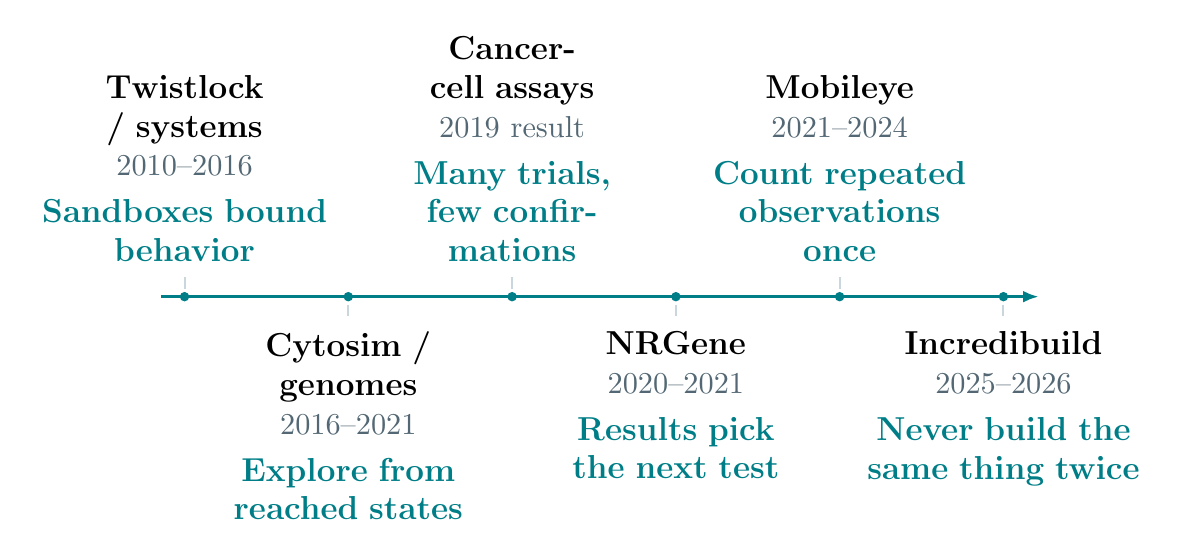
\begin{tikzpicture}[x=1cm,y=1cm,every node/.style={align=center},
  stop/.style={text width=3.62cm,font=\fontsize{11.5}{14}\selectfont}]
\draw[-{Latex[length=2mm]},Teal,line width=1.2pt](-.3,0)--(10.85,0);
\foreach \x in {0,2.08,4.16,6.24,8.32,10.4}{\fill[Teal](\x,0)circle(.06cm);}
\foreach \x in {0,4.16,8.32}{\draw[Line,line width=.7pt](\x,.1)--(\x,.25);}
\foreach \x in {2.08,6.24,10.4}{\draw[Line,line width=.7pt](\x,-.1)--(\x,-.25);}
\node[stop,anchor=south,text width=3.75cm]at(0,.32){\textbf{Twistlock / systems}\\{\fontsize{10.5}{12.5}\selectfont\color{Muted}2010--2016}\\[3pt]{\color{Teal}\bfseries Sandboxes bound\\behavior}};
\node[stop,anchor=north]at(2.08,-.32){\textbf{Cytosim / genomes}\\{\fontsize{10.5}{12.5}\selectfont\color{Muted}2016--2021}\\[3pt]{\color{Teal}\bfseries Explore from\\reached states}};
\node[stop,anchor=south]at(4.16,.32){\textbf{Cancer-cell assays}\\{\fontsize{10.5}{12.5}\selectfont\color{Muted}2019 result}\\[3pt]{\color{Teal}\bfseries Many trials,\\few confirmations}};
\node[stop,anchor=north]at(6.24,-.32){\textbf{NRGene}\\{\fontsize{10.5}{12.5}\selectfont\color{Muted}2020--2021}\\[3pt]{\color{Teal}\bfseries Results pick\\the next test}};
\node[stop,anchor=south]at(8.32,.32){\textbf{Mobileye}\\{\fontsize{10.5}{12.5}\selectfont\color{Muted}2021--2024}\\[3pt]{\color{Teal}\bfseries Count repeated\\observations once}};
\node[stop,anchor=north]at(10.4,-.32){\textbf{Incredibuild}\\{\fontsize{10.5}{12.5}\selectfont\color{Muted}2025--2026}\\[3pt]{\color{Teal}\bfseries Never build the\\same thing twice}};
\end{tikzpicture}\end{center}
\sources{\href{https://yossieliaz.netlify.app/}{Career periods}; \href{https://doi.org/10.1038/s41598-019-51537-7}{cancer-drug result (2019)}. Periods overlap; not to scale. Lessons are my reading, not results.}
\qadetail{Chronology follows the speaker's own career website, retrieved 4 October 2026: the 2010--2016 band groups Twistlock, Broadcom, Marvell and BAE Systems/Rokar, rather than six years of employment at Twistlock alone. Twistlock's January 2017 vendor account describes per-image process, filesystem, network and system-call learning and enforcement; prior employment does not attribute every feature to the speaker. The 2016--2021 research band is Baylor College of Medicine and Rice University: Cytosim actomyosin simulations and genomics research; the University of Houston Physics PhD was awarded in 2020. The dated 2019 event is the published PD-L1/cytotoxicity combination study, DOI 10.1038/s41598-019-51537-7, rather than an employment transition or clinical immunotherapy system. NRGene ran August 2020--November 2021; its CRISPR-IL/GoGenome architecture account with Noam Barkai was published in February 2022. Mobileye ran December 2021--March 2024, with deep-learning work on production perception and road-junction semantics. Incredibuild/islo.dev began December 2025 and continues in 2026. Bands overlap; milestone spacing is for reading, not a linear time scale. Harvard Medical School computational biology, March 2024--January 2026, and Matia ML/AI product work, March--August 2025, are additional overlapping roles retained here as context rather than additional on-slide stops. The teal lessons are the speaker's retrospective framing of each stop, not findings of those projects. Local physical self-organization is not goal-directed agency. Researcher-led gene-editing feedback and cancer-cell assays do not establish autonomous genetic engineering or adaptive clinical treatment. Scientific results retain coauthor attribution. The final compute stage is a proposed integration of reusable state, external evidence and controller authority, with the exercised components distinguished later in the deck.}
\note{[0:55] Here is my path, and each stop left one lesson. In early systems jobs, including Twistlock, I worked on software and container security: a sandbox bounds what a program may do. From twenty sixteen I simulated cell mechanics and analyzed genomes, where reaching a state is the expensive part, so you explore from there. Our twenty nineteen study tested drug combinations on cancer cells: many trials, few confirmations. At NRGene, editing results helped pick the next test. At Mobileye, repeated observations of one road had to count once. And at Incredibuild, the rule is simple: never build the same thing twice. These lessons come back later. Mobileye first.}
\end{frame}

% Act 1: the Mobileye fleet as the fan-out/fan-in picture; the map counts each road once (rule two).
\begin{frame}[t]{\ev{\tagO\,\tagP}A car fleet fans out, then fans in to one map.}
\vspace{.05cm}
\begin{columns}[T,onlytextwidth]
\column{.45\linewidth}
\vspace{.2cm}
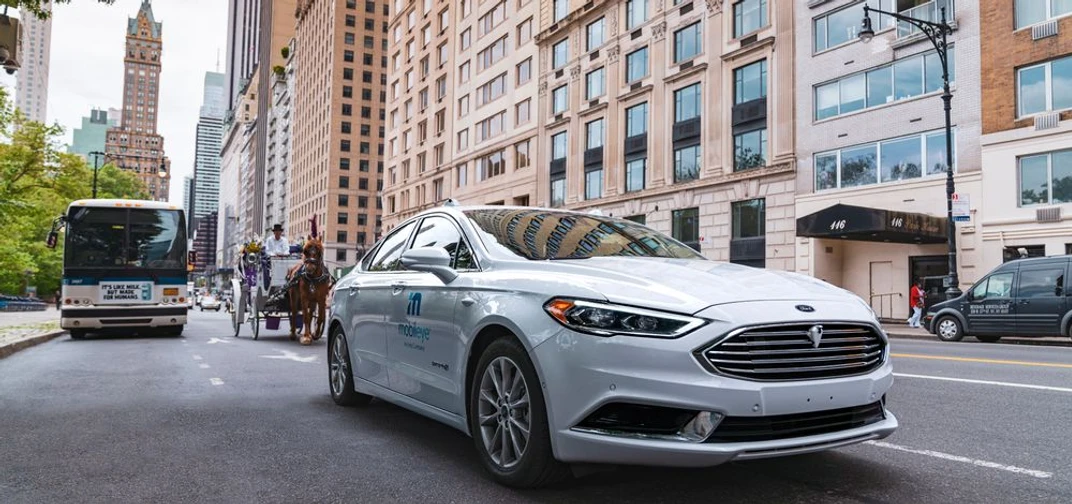
\includegraphics[width=\linewidth]{assets/mobileye-new-york-2021.png}\par
\tagline{Mobileye autonomous test vehicle,\\Manhattan, June 2021.}
\vspace{.12cm}
{\fontsize{11}{13}\selectfont\textbf{My work, 2021--2024:}\\junction perception.\par}
\column{.51\linewidth}
{\centering
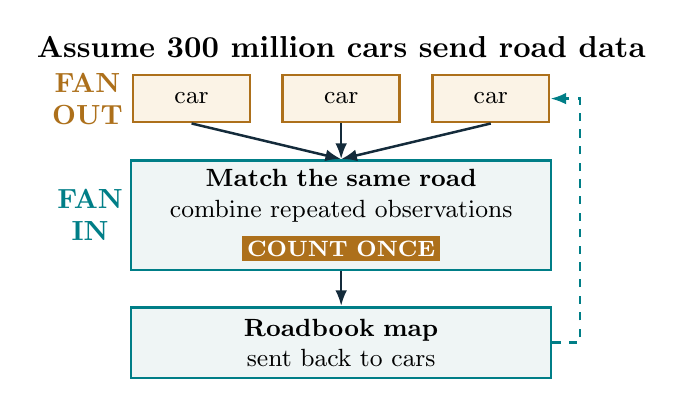
\begin{tikzpicture}[x=1cm,y=1cm,every node/.style={align=center,font=\fontsize{11}{13}\selectfont}, side/.style={font=\fontsize{10}{11.5}\selectfont\bfseries,anchor=east}]
\node[font=\fontsize{11}{13}\selectfont\bfseries] at (0,3.25) {Assume 300 million cars send road data};
\foreach \k/\x in {1/-1.9,2/0,3/1.9}{\node[candidate,text width=1.25cm,minimum height=.6cm](c\k)at(\x,2.6){car};}
\node[evidence,text width=5.1cm,minimum height=.9cm](m)at(0,1.12){\textbf{Match the same road}\\combine repeated observations\\[3pt]{\setlength{\fboxsep}{1.7pt}\colorbox{Gold}{\textcolor{white}{\fontsize{7.6}{8.6}\selectfont\bfseries COUNT ONCE}}}};
\node[evidence,text width=5.1cm,minimum height=.9cm](r)at(0,-.5){\textbf{Roadbook map}\\sent back to cars};
\foreach \k in {1,2,3}{\draw[flow](c\k.south)--(m.north);}
\draw[flow](m)--(r);
\draw[message](r.east)--++(.35,0)|-(c3.east);
\node[side,text=Gold]at(-2.65,2.6){FAN\\OUT};
\node[side,text=Teal]at(-2.65,1.12){FAN\\IN};
\end{tikzpicture}\par}
\end{columns}
\claim{Self-driving compute: many runs from one state, one combined result.}
\sources{300M fleet: speaker-reported. \href{https://ir.mobileye.com/news-releases/news-release-details/mobileye-supply-cloud-enhanced-adas-select-future-stellantis}{Anonymized data flow}; \href{https://www.mobileye.com/technology/rem/}{Roadbook workflow}. Photo: \href{https://www.mobileye.com/press-kit/press-kit-mobileye-new-york-city/}{Mobileye press kit}.}
\qadetail{Fleet wording follows the speaker's request of 4 October 2026: assume 300 million Mobileye-equipped cars sensing roads and transmitting anonymized road data. The figure is supplied by the speaker from firsthand Mobileye experience and remains visibly attributed; it is not an independently verified public contributor count. The official 21 July 2026 release supports anonymized road-feature transmission to the cloud, processing and feedback to vehicles. That release reports a different, narrower mapping population: over eight million contributing vehicles and 34 billion road-miles in 2025 (about 1,080 road-miles per second as an annual average), alongside over 230 million vehicles built with EyeQ through 2025. These populations and dates do not establish a measured rate for the assumed 300-million-car fleet; no per-car transmission rate is asserted. The Roadbook workflow aligns repeated observations from the same road before combining them into a high-definition map of lanes, signs and driving paths and returning updates to cars. The COUNT ONCE chip is the talk's reading of that alignment step (many drives of one road are not independent roads), not a claim about Mobileye's statistical model. Parallel collection and aggregation motivate the computational fan-out/fan-in analogy without treating cars as checkpoint clones or repeated observations as independent evidence. The pictured vehicle is an autonomous test vehicle from Mobileye's Manhattan fleet, June 2021, as identified by the official press kit; it is not attributed to the speaker's team. The speaker's Mobileye employment, December 2021--March 2024, covered deep learning for production perception and road-junction semantics; personal junction-perception work is not authorship of the fleet mapping system. No Mobileye production accuracy or safety metric is asserted. The photo is the official image converted losslessly to PNG and scaled proportionally.}
\note{[0:45] Mobileye's Roadbook is a fleet example. Assume three hundred million equipped cars sending anonymized road observations. The cloud matches drives on the same road, combines them, and sends the updated map back to the cars. My own work there was junction perception. Notice that the map counts each road once, however many cars drove it. That is rule two. Self-driving compute gives execution the same shape: many runs from one reached state, one combined result.}
\end{frame}

% Act 1: the oldest form of not doing work twice; the hash that keys the cache starts the content-identity thread.
\begin{frame}[t]{\ev{\tagO\,\tagM}A cache skips work that a previous run did.}
\vspace{.15cm}
\begin{columns}[T,onlytextwidth]
\begin{column}{.56\textwidth}
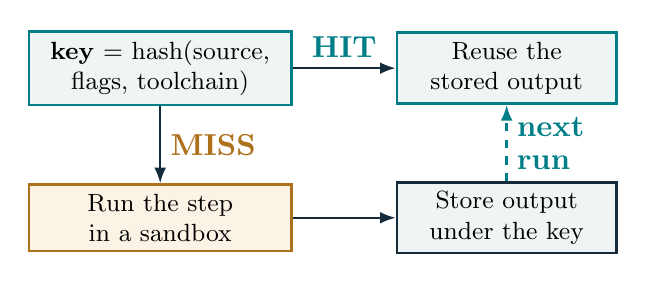
\begin{tikzpicture}[x=1cm,y=1cm,every node/.style={align=center,font=\fontsize{11.5}{14}\selectfont}, lab/.style={font=\fontsize{10.5}{12}\selectfont\bfseries}]
\node[evidence,text width=3.1cm] (k) at (1.6,0) {\textbf{key} $=$ hash(source,\\flags, toolchain)};
\node[evidence,text width=2.55cm] (hit) at (6.0,0) {Reuse the\\stored output};
\node[candidate,text width=3.1cm] (run) at (1.6,-1.9) {Run the step\\in a sandbox};
\node[state,text width=2.55cm] (st) at (6.0,-1.9) {Store output\\under the key};
\draw[flow] (k)--node[above,lab,text=Teal]{HIT}(hit);
\draw[flow] (k)--node[right,lab,text=Gold]{MISS}(run);
\draw[flow] (run)--(st);
\draw[message] (st)--node[right,lab,text=Teal,align=left]{next\\run}(hit);
\end{tikzpicture}
\par\vspace{.2cm}
{\fontsize{11.5}{14}\selectfont The sandbox hides undeclared files,\\so a step cannot read what the key omits.\par}
\end{column}
\begin{column}{.40\textwidth}
{\fontsize{9.5}{11}\selectfont\color{Teal}\bfseries TOKIO COMPILE\par}
\vspace{.2cm}
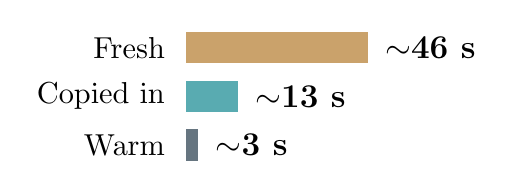
\begin{tikzpicture}[x=1cm,y=1cm,every node/.style={font=\fontsize{11}{13}\selectfont}]
\foreach \blabel/\seconds/\y/\col in {Fresh/46/0/Gold,Copied in/13/-.62/Teal,Warm/3/-1.24/Ink}{
\node[anchor=east,align=right] at (1.55,\y+.2) {\blabel};
\fill[\col!65] (1.7,\y) rectangle ({1.7+\seconds*.05},\y+.4);
\node[anchor=west,font=\fontsize{12.5}{15}\selectfont\bfseries] at ({1.8+\seconds*.05},\y+.2) {$\sim$\seconds\ s};}
\end{tikzpicture}
\par\vspace{.2cm}
{\fontsize{10.5}{12.5}\selectfont\color{Muted}Copied in: an earlier runner's build files, not its running state.\par}
\end{column}
\end{columns}
\claim{Distributed builds rely on it: one machine reuses another's output.}
\sources{Tokio: Eliaz, \href{https://github.com/tokio-rs/tokio/issues/8200}{issue \#8200}, 8 June 2026; author-reported external Incredibuild demo, approximate compile times.}
\qadetail{The left diagram is the generic content-addressed action cache used by ccache, Bazel remote caching and Incredibuild: the key is a hash of the declared inputs (sources, flags, toolchain); a hit reuses the stored output; a miss runs the step and stores its output under the key. Sandboxing (hermetic execution) hides undeclared files, so a step cannot silently depend on inputs the key omits; time, randomness, network and nondeterministic tools still need declaring or excluding, so the key covers every input only when the step is hermetic. The hash proves identity of inputs, not correctness of outputs. Tokio: restored cache means Incredibuild compiler artifacts persisted across fresh GitHub Actions runners; hot (already warm) cache denotes the already available cache state in the reported demo. Author-reported external Incredibuild GitHub Actions demo, posted by zozo123 in Tokio issue 8200 on 8 June 2026; approximate compile endpoints 46 s fresh, 13 s restored, 3 s hot. No controlled raw benchmark protocol is posted, and no maintainer adoption is claimed. The issue does not publish enough configuration to isolate disk artifacts, memory/page cache, cache lookup, transfer or incremental checking costs; do not attribute the 13-to-3-second difference entirely to download time or OS memory. Full test path approximately 75 s fresh and 43 s restored; Cargo after touching source approximately 38 s versus 13 s restored Incredibuild. These are static artifact-cache endpoints, not memory-checkpoint or fork timings; the slide labels the issue's restored cache as copied in so that it is not read as restoring execution state, which slide 17 prices. Bazel's local sandbox hides undeclared workspace files, but system directories typically stay visible read-only; hermetic toolchains or a pinned remote-execution image close that gap. We do not claim that a fork is faster than a good build cache.}
\note{[1:05] Start with the oldest way to avoid doing work twice: a cache. Hash a build step's inputs, the source, the flags and the toolchain, into a key. If the key is stored, that is a hit: reuse the stored output. On a miss, run the step in a sandbox and store its output under the key. The sandbox hides files the step did not declare, so it cannot read what the key leaves out. This is the Incredibuild lesson. In my Tokio demo, a fresh compile took about forty-six seconds, copying in an earlier runner's build files about thirteen, and an already warm cache about three. Distributed builds rely on this: one machine reuses another's output. Remember that hash; it comes back.}
\end{frame}

% Act 1: from a cached step to a reached state; each alternative runs in a private sandbox.
\begin{frame}[t]{\ev{\tagP}A fork extends caching from files to a reached execution state.}
\vspace{.05cm}
{\fontsize{12.5}{15}\selectfont\textbf{Cache:} one step's output.\qquad\textcolor{Teal}{\textbf{Fork:} the state after many steps.}\par}
{\fontsize{10.5}{12.5}\selectfont\color{Muted}Installed dependencies, a reproduced failure, a warmed process.\par}
\vspace{.05cm}
\begin{center}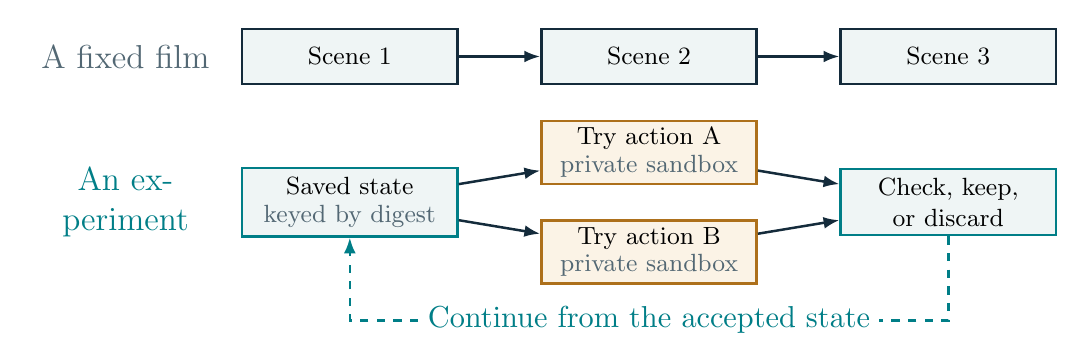
\begin{tikzpicture}[x=1cm,y=1cm,every node/.style={align=center,font=\fontsize{12}{14.5}\selectfont}]
\node[text=Muted,anchor=east,text width=2.25cm] at (-.3,0) {A fixed film};
\node[state,text width=2.5cm,minimum height=.7cm](s)at(1.3,0){Scene 1};
\node[state,text width=2.5cm,minimum height=.7cm](t)at(5.1,0){Scene 2};
\node[state,text width=2.5cm,minimum height=.7cm](u)at(8.9,0){Scene 3};
\draw[flow](s)--(t);\draw[flow](t)--(u);
\node[text=Teal,anchor=east,text width=2.25cm] at (-.3,-1.85) {An experiment};
\node[evidence,text width=2.5cm](saved)at(1.3,-1.85){Saved state\\[-1pt]{\fontsize{9.5}{11}\selectfont\color{Muted}keyed by digest}};
\node[candidate,text width=2.5cm,inner ysep=2pt](a)at(5.1,-1.22){Try action A\\[-1pt]{\fontsize{9.5}{11}\selectfont\color{Muted}private sandbox}};
\node[candidate,text width=2.5cm,inner ysep=2pt](b)at(5.1,-2.48){Try action B\\[-1pt]{\fontsize{9.5}{11}\selectfont\color{Muted}private sandbox}};
\node[evidence,text width=2.5cm](choose)at(8.9,-1.85){Check, keep,\\or discard};
\draw[flow](saved)--(a);\draw[flow](saved)--(b);
\draw[flow](a)--(choose);\draw[flow](b)--(choose);
\draw[message](choose.south)--++(0,-1.07)-|(saved.south);
\node[text=Teal,font=\fontsize{10.5}{12}\selectfont,fill=white,inner ysep=1pt]at(5.1,-3.34){Continue from the accepted state};
\end{tikzpicture}\end{center}
\sources{Organizing analogy and proposed execution model. Stored-program hardware remains the substrate.}
\qadetail{Cache versus fork: both are reuse, and both need a key. Proposed: the parent is immutable and named by its digest; a child is that digest plus its private delta. Changing an input that reached the parent needs a new parent, as a cache miss would. The islo snapshots we measured are named snapshots; we do not claim they are content-addressed today. A cache returns one step's stored output, keyed by its inputs; a fork restores a captured execution state and lets several private continuations diverge from it. Which state a fork must capture depends on the next action: files and cached inputs, or supported memory and runtime state. Installed dependencies are file state; a reproduced failure in a running application is a hypothetical future live-state workload, not an observed property of our factory runs; a warmed process requires a process or VM checkpoint whose memory semantics must be checked. The comparison priced later is restoring saved state versus rebuilding with a warm cache; we do not claim that a fork is faster than a good build cache. Von Neumann is a hardware and stored-program architectural model. Adaptive planning, search, operating-system process fork and feedback control have long histories. The claim is an organizing research direction combining reusable execution with adaptive orchestration, not historical priority, a replacement ISA or new computational expressive power. Forkability and autonomy are separable: a runtime may fork without an agent, and an agent may operate serially without forks. The film analogy refers to private executable continuations from saved computer state. It does not rewind completed model or tool requests, incurred costs, published data or other external-world effects, and restoring a snapshot does not establish a child's current authority.}
\note{[0:50] A cache reuses one step's output. A fork goes further: it reuses the state after many steps, such as installed dependencies, a reproduced failure or a warmed process. Think of a film: a fixed sequence of scenes, and rewinding replays the same plot. Now save a reached state and try two different next actions, each in its own private sandbox. A check decides which outcome to keep; the other is discarded, and we continue from the accepted state. Like a cache entry, the saved state needs a key: the parent's digest. Here is the same idea as code.}
\end{frame}

% Act 1: the same three edits as a plain loop and as a proposed forkable API; prepare() is the repeated work.
\begin{frame}[fragile,t]{\ev{\tagP}The forkable API prepares once and runs alternatives in private children.}
\vspace{-.12cm}
\lead{Same three edits, same test, same selection rule.}
\begin{columns}[T,onlytextwidth]
\column{.47\textwidth}
{\fontsize{14}{17}\selectfont\bfseries Python loop\par}
\begin{lstlisting}[style=slidepython]
out = []
for edit in edits:
    env = prepare()
    env.apply(edit)
    out.append(test(env))
best = select(out)
\end{lstlisting}
\column{.49\textwidth}
{\fontsize{14}{17}\selectfont\bfseries\color{Teal}Forkable API\par}
\begin{lstlisting}[style=slidepython]
parent = checkpoint(prepare())
children = fork(parent, n=3)
execute(children, edits)
out = evaluate(children, test)
best = select(out)
\end{lstlisting}
\end{columns}
\vspace{.12cm}
\begin{columns}[T,onlytextwidth]
\column{.47\textwidth}
{\fontsize{12.5}{15}\selectfont\color{Muted}\texttt{prepare()} \textbf{3} times.\par}
\column{.49\textwidth}
{\fontsize{12.5}{15}\selectfont\color{Teal}\texttt{prepare()} \textbf{once}; \textbf{3} private children.\par}
\end{columns}
\sources{Proposed API sketch, not an existing SDK. Both columns are Python; each check returns its artifact and evidence.}
\qadetail{The snippets illustrate a proposed API surface, not an existing SDK or a claim that these exact signatures are implemented. Both operate on the same three-element edits list, equivalent prepared input state, the same test function and the same select function. On the left, each iteration prepares a new environment, applies one edit and collects a test result. On the right, checkpoint captures the required reached state, fork creates three private writable children, execute applies one edit per child and evaluate invokes the same test in each child. Result records identify their child, exact artifact and evidence. select applies the same selection rule in both sketches; it is not an infallible verifier and not the built numerical reducer. No concurrency or speedup value is asserted. Ordinary Python can use process fork, worktrees or warm caches to avoid repeated preparation; the interface adds no computational expressive power. The explicit API makes captured state and private continuations first-class orchestration objects; useful-state validity, code reload/restart, external effects, private writes and controller authority require their declared semantics.}
\note{[0:50] Both columns are Python. They try the same three edits, with the same test and the same selection rule. The loop prepares a fresh environment for every edit. The proposed API prepares once, checkpoints that state and forks three private children; each child applies one edit and returns its result with evidence. prepare() is the work we stop doing three times. Ordinary Python can already do this with process forks or caches; the API makes reuse and isolation explicit. None of these pieces is new on its own.}
\end{frame}

% Act 1: fence the idea -- what is old (the three mechanisms) and what is new (coupling reuse with evidence and acceptance).
\begin{frame}[t]{\ev{\tagO}Caches, forks and sandboxes are old; coupling them to evidence and acceptance is new.}
\vspace{0pt}
{\fontsize{11}{13.2}\selectfont\renewcommand{\arraystretch}{1.0}
\begin{tabularx}{\linewidth}{@{}L{1.75cm}L{3.3cm}L{3.6cm}Y@{}}
\toprule
 & \textcolor{Teal}{\textbf{Reuses or protects}} & \textcolor{Teal}{\textbf{Must guarantee}} & \textcolor{Teal}{\textbf{Known systems}}\\
\midrule
\textbf{Cache} & a run's output & key covers all inputs & \textcolor{Muted}{ccache, Bazel remote cache, Incredibuild}\\\addlinespace[3pt]
\textbf{Fork} & a reached state & capture keeps what the next step needs & \textcolor{Muted}{SnowFlock on Xen (2009), CRIU, Firecracker snapshots}\\\addlinespace[3pt]
\textbf{Sandbox} & reads and writes & undeclared inputs hidden; writes private & \textcolor{Muted}{containers, gVisor, microVMs}\\
\bottomrule
\end{tabularx}\par}
\claim{New: count shared evidence once; publish checked bytes once.}
\vspace{.12cm}
{\fontsize{10.5}{12.8}\selectfont\color{Muted}\textbf{Not claimed today:} a fork speedup (our agent runs were serial), or live-memory restore.\par}
\sources{SnowFlock: Lagar-Cavilla et al., EuroSys 2009. Firecracker: Agache et al., NSDI 2020. CRIU, gVisor, ccache, Bazel.}
\qadetail{The table names established mechanisms; no claim of invention, comprehensive priority or measured parallel speedup is made. Forking states to search is also old: KLEE (Cadar, Dunbar and Engler, OSDI 2008) and S2E (Chipounov, Kuznetsov and Candea, ASPLOS 2011) fork execution states; the AFL forkserver forks an initialized target per input; Potemkin (Vrable et al., SOSP 2005) flash-clones VMs. The claim is the evidence and acceptance contract around reuse, not search by forking. The contribution claim is the integrated execution, evidence and acceptance contract: reuse a state only when it beats rebuilding it, count shared observations once, and publish the exact checked bytes once from a controller. Cache guarantees hold only for hermetic steps: time, randomness, network and undeclared files must be declared or excluded. Fork semantics are backend-specific: worktrees preserve source views, process checkpoints (CRIU, gVisor save/restore) and VM snapshots (Xen, SnowFlock, Firecracker) preserve only their declared state surfaces, and filesystem snapshots do not establish memory capture. SnowFlock: Lagar-Cavilla et al., Rapid Virtual Machine Cloning for Cloud Computing, EuroSys 2009, built on Xen; Xen came from the Cambridge Computer Laboratory (Barham et al., SOSP 2003). A sandbox bounds local effects; it does not undo remote effects, and a restored child must not hold publication authority. Not claimed: our factory runs (SELFHOST-2 and SELFHOST-3, 27 September 2026) ran serially in Docker Sandboxes, not islo, and nothing forked, so no fork speedup is measured; we do not claim that a fork is faster than a good build cache. Restore fan-out means many restores of one named snapshot: a named 141 MB islo snapshot, restore--run--capture round trips, 255 of 256 succeeded at concurrency 12, p50 6.87 s, p95 9.04 s, client-measured, teardown excluded (arXiv:2607.09689v4, Table 2). These are API round trips, not mechanism latency. Memory preservation is unverified until the preregistered Gate 0 RAM-nonce probe runs, so no islo snapshot is described as a memory fork.}
\note{[1:00] Let me fence the idea: the mechanisms are old. A cache reuses a run's output; its key must cover every input, as in ccache or Bazel's remote cache. A fork reuses a reached state, and capture must keep what the next step needs. SnowFlock forked Xen machines in two thousand nine; Xen came from this lab. A sandbox hides undeclared inputs and keeps each trial's writes private. Even forking for search is old; fuzzers do it. What is new is coupling reuse with evidence and acceptance: count once, publish once. I do not claim a fork speedup, since our agent runs were serial, or that our snapshots keep memory: we restore one snapshot many times. Now the examples.}
\end{frame}

\setact{2}
% Act 2 example: shared template for short/10--14 (same geometry; only text and rule chips change).
% Rule chip: gold, right-aligned on the claim line; names match the map columns on slides 3, 15 and 26.
\providecommand{\exchip}[1]{\tikz[baseline=(x.base)]\node[fill=Gold,text=white,rounded corners=1.5pt,inner xsep=2.6pt,inner ysep=1.7pt,font=\fontsize{7.6}{8.6}\selectfont\bfseries](x){#1};}
\begin{frame}[t]{\ev{\tagO}\surf{SOFTWARE SECURITY}Reuse makes fuzzing fast; only checks turn crashes into findings.\strut}
\vspace{.15cm}
\noindent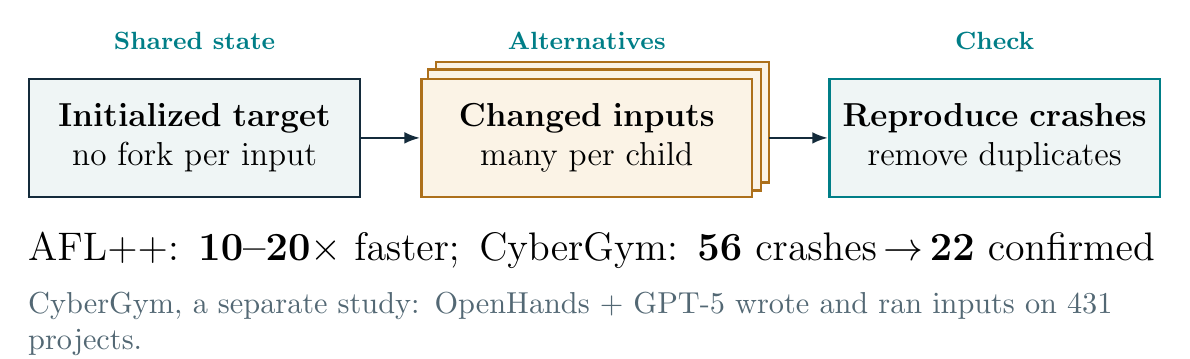
\begin{tikzpicture}[x=1cm,y=1cm,
  hd/.style={anchor=south,font=\fontsize{9.5}{11}\selectfont\bfseries,text=Teal},
  bx/.style={text width=3.9cm,inner xsep=.15cm,minimum height=1.5cm,font=\fontsize{11.5}{14}\selectfont},
  stack/.style={draw=Gold,fill=Sand,line width=.9pt},
  res/.style={anchor=north west,inner sep=0pt,text width=14.4cm,align=left,font=\fontsize{14.5}{17.5}\selectfont},
  ctx/.style={anchor=north west,inner sep=0pt,text width=14.4cm,align=left,font=\fontsize{10.5}{13}\selectfont,text=Muted},
  every node/.style={align=center}]
\useasboundingbox (0,.55) rectangle (14.4,-3.3);
\node[hd] at (2.12,.15) {Shared state};
\node[hd] at (7.10,.15) {Alternatives};
\node[hd] at (12.28,.15) {Check};
\node[state,bx] (s) at (2.12,-.85) {\textbf{Initialized target}\\no fork per input};
\node[candidate,bx] (a) at (7.10,-.85) {\textbf{Changed inputs}\\many per child};
\begin{scope}[on background layer]
\draw[stack] ($(a.south west)+(.2,.2)$) rectangle ($(a.north east)+(.2,.2)$);
\draw[stack] ($(a.south west)+(.1,.1)$) rectangle ($(a.north east)+(.1,.1)$);
\end{scope}
\node[evidence,bx] (c) at (12.28,-.85) {\textbf{Reproduce crashes}\\remove duplicates};
\draw[flow] (s.east)--(a.west);
\draw[flow] ($(a.east)+(.2,0)$)--(c.west);
\node[res] at (0,-2.05) {AFL++: \textbf{10--20$\times$} faster;\enspace CyberGym: \textbf{56} crashes\,$\to$\,\textbf{22} confirmed};
\node[ctx] at (0,-2.8) {CyberGym, a separate study: OpenHands + GPT-5 wrote and ran inputs on 431 projects.};
\end{tikzpicture}
\claim{Set up the target once; count each bug once.\hspace{.8em}\hfill\exchip{COMPUTE ONCE}\enspace\exchip{COUNT ONCE}}
\sources{\href{https://github.com/AFLplusplus/AFLplusplus/blob/stable/instrumentation/README.persistent_mode.md}{AFL++ persistent-mode docs}, typical gain vs a fork per input; \href{https://www.cybergym.io/cybergym/}{CyberGym report}, latest-code GPT-5 campaign.}
\qadetail{Two separate sources: AFL++ documentation supplies the speed figure; CyberGym is a separate agent study that does not claim AFL++ or persistent-mode reuse. AFL++: the documented typical 10--20x gain is for persistent mode, which avoids a process fork for every input; it must not be attributed solely to the deferred forkserver. The forkserver defers cloning until initialization is complete; a persistent child then runs the harness repeatedly, resetting mutable state between inputs. About 1,000 iterations before restarting is a recommended starting point, not a fixed setting. Gains depend on the target and reset correctness. A newly executed input is not automatically an independent observation, and a crash is not automatically an exploitable vulnerability. CyberGym latest-code campaign (report checked 4 October 2026): OpenHands with GPT-5 on 431 latest OSS-Fuzz projects and 1,748 runnable executables produced 56 crashes; the authors reproduced, deduplicated and investigated them, confirming 22 distinct previously unknown vulnerabilities. Projects, targets, crashes and validated bugs are different units; the funnel is not a disjoint 22/56 success probability, and exploitability or patch status is not implied. This is separate from CyberGym's historical 1,507-vulnerability benchmark across 188 projects. The separate GPT-4.1 campaign's counts overlap and cannot be added. Neither result measures sandbox forking or our own security campaign.}
% Transition: Duplicates count once; the same loop next runs on training code.
\note{[1:05] Five examples, one loop: a shared state, many alternatives, one check. We go from systems toward science. First, security. AFL-plus-plus, a fuzzer, initializes the target once and reuses one child across many changed inputs. Its documentation reports typical speedups of ten to twenty times in persistent mode. Notice it wins by not forking for every input, as long as state resets correctly. That is rule one, compute once, and it returns in the runtime section. Speed produces leads, and leads need checks. In a separate study, Berkeley's CyberGym, an AI agent wrote and ran inputs against 431 projects and produced fifty-six crashes. Researchers reproduced them and removed duplicates: twenty-two distinct new vulnerabilities. Rule two, count once. Next, the same loop in AI research.}
\end{frame}

% Act 2 example: shared template for short/10--14 (same geometry; only text and rule chips change).
% Rule chip: gold, right-aligned on the claim line; names match the map columns on slides 3, 15 and 26.
\providecommand{\exchip}[1]{\tikz[baseline=(x.base)]\node[fill=Gold,text=white,rounded corners=1.5pt,inner xsep=2.6pt,inner ysep=1.7pt,font=\fontsize{7.6}{8.6}\selectfont\bfseries](x){#1};}
\begin{frame}[t]{\ev{\tagO}\surf{AI RESEARCH}Autoresearch kept 23 of 126 attempts against a fixed evaluator.\strut}
\vspace{.15cm}
\noindent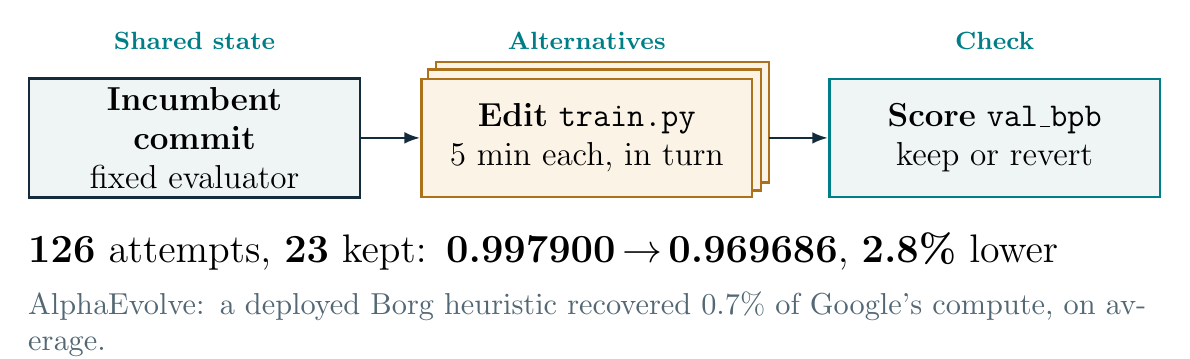
\begin{tikzpicture}[x=1cm,y=1cm,
  hd/.style={anchor=south,font=\fontsize{9.5}{11}\selectfont\bfseries,text=Teal},
  bx/.style={text width=3.9cm,inner xsep=.15cm,minimum height=1.5cm,font=\fontsize{11.5}{14}\selectfont},
  stack/.style={draw=Gold,fill=Sand,line width=.9pt},
  res/.style={anchor=north west,inner sep=0pt,text width=14.4cm,align=left,font=\fontsize{14.5}{17.5}\selectfont},
  ctx/.style={anchor=north west,inner sep=0pt,text width=14.4cm,align=left,font=\fontsize{10.5}{13}\selectfont,text=Muted},
  every node/.style={align=center}]
\useasboundingbox (0,.55) rectangle (14.4,-3.3);
\node[hd] at (2.12,.15) {Shared state};
\node[hd] at (7.10,.15) {Alternatives};
\node[hd] at (12.28,.15) {Check};
\node[state,bx] (s) at (2.12,-.85) {\textbf{Incumbent commit}\\fixed evaluator};
\node[candidate,bx] (a) at (7.10,-.85) {\textbf{Edit \texttt{train.py}}\\5 min each, in turn};
\begin{scope}[on background layer]
\draw[stack] ($(a.south west)+(.2,.2)$) rectangle ($(a.north east)+(.2,.2)$);
\draw[stack] ($(a.south west)+(.1,.1)$) rectangle ($(a.north east)+(.1,.1)$);
\end{scope}
\node[evidence,bx] (c) at (12.28,-.85) {\textbf{Score \texttt{val\_bpb}}\\keep or revert};
\draw[flow] (s.east)--(a.west);
\draw[flow] ($(a.east)+(.2,0)$)--(c.west);
\node[res] at (0,-2.05) {\textbf{126} attempts, \textbf{23} kept:\enspace \textbf{0.997900}\,$\to$\,\textbf{0.969686}, \textbf{2.8\%} lower};
\node[ctx] at (0,-2.8) {AlphaEvolve: a deployed Borg heuristic recovered 0.7\% of Google's compute, on average.};
\end{tikzpicture}
\claim{Reuse the incumbent; the evaluator promotes.\hspace{.8em}\hfill\exchip{COMPUTE ONCE}\enspace\exchip{PUBLISH ONCE}}
\sources{\href{https://github.com/karpathy/autoresearch/blob/master/program.md}{Karpathy, autoresearch protocol}; \href{https://github.com/karpathy/autoresearch/discussions/43}{reported session}. \href{https://deepmind.google/blog/alphaevolve-a-gemini-powered-coding-agent-for-designing-advanced-algorithms/}{Google DeepMind, AlphaEvolve (2025)}.}
\qadetail{Autoresearch: one reported session, not a controlled average effect or a fork experiment. 126 attempts: 23 kept, 102 discarded, 1 crash. The score decline is (0.997900-0.969686)/0.997900=2.827\%; lower validation bits per byte is better. The protocol holds data preparation, tokenizer and evaluation fixed and permits editing train.py. Five minutes is wall-clock training time; startup and compilation are outside that budget, and crashes can end early. Sequential Git keep/revert is the actual mechanism; forked parallel continuations are a possible extension, not what produced this result. Repeated adaptive selection on one validation set warrants a separate held-out check before claiming generalization. AlphaEvolve: DeepMind reports that the discovered Borg scheduling heuristic recovered an average 0.7\% of Google's worldwide compute resources, in production for over a year at announcement. A separate kernel result (23\% kernel speedup, 1\% lower Gemini training time) is a different workload and endpoint; the gains are not additive. Gemini Flash and Pro propose edits; automated evaluators check validity and performance; evolutionary selection keeps useful programs. The gains belong to the discovered algorithms, not to a sandbox fork or our implementation.}
% Transition: One attempt at a time here; the next example samples many patches from one repository.
\note{[1:05] Second, AI research. Karpathy's autoresearch starts every attempt from the incumbent commit, and the commit hash names that exact state. The evaluator stays fixed. The agent edits the training script, trains for five minutes, reads validation bits per byte, then keeps or reverts. One reported session made 126 attempts, one at a time, and kept twenty-three. The score fell by 2.8 percent. Starting from the incumbent is compute once; only the fixed evaluator promotes a change, which is publish once. AlphaEvolve runs this loop over a population of programs; a scheduling heuristic it found recovered 0.7 percent of Google's compute, on average. Tuned on one validation set, a result still needs a held-out check. Next, many attempts from one repository.}
\end{frame}

% Act 2 example: shared template for short/10--14 (same geometry; only text and rule chips change).
% Rule chip: gold, right-aligned on the claim line; names match the map columns on slides 3, 15 and 26.
\providecommand{\exchip}[1]{\tikz[baseline=(x.base)]\node[fill=Gold,text=white,rounded corners=1.5pt,inner xsep=2.6pt,inner ysep=1.7pt,font=\fontsize{7.6}{8.6}\selectfont\bfseries](x){#1};}
\begin{frame}[t]{\ev{\tagO}\surf{SOFTWARE ENGINEERING}250 samples raised SWE-bench Lite coverage from 15.9\% to 56\%.\strut}
\vspace{.15cm}
\noindent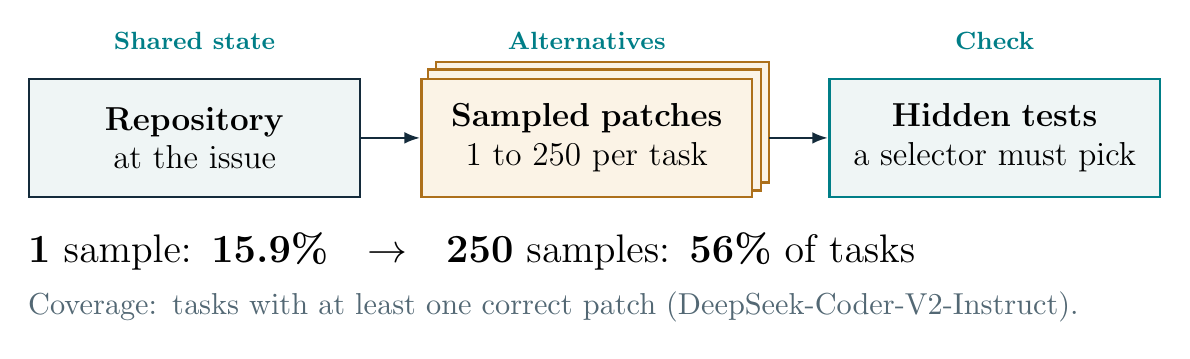
\begin{tikzpicture}[x=1cm,y=1cm,
  hd/.style={anchor=south,font=\fontsize{9.5}{11}\selectfont\bfseries,text=Teal},
  bx/.style={text width=3.9cm,inner xsep=.15cm,minimum height=1.5cm,font=\fontsize{11.5}{14}\selectfont},
  stack/.style={draw=Gold,fill=Sand,line width=.9pt},
  res/.style={anchor=north west,inner sep=0pt,text width=14.4cm,align=left,font=\fontsize{14.5}{17.5}\selectfont},
  ctx/.style={anchor=north west,inner sep=0pt,text width=14.4cm,align=left,font=\fontsize{10.5}{13}\selectfont,text=Muted},
  every node/.style={align=center}]
\useasboundingbox (0,.55) rectangle (14.4,-3.3);
\node[hd] at (2.12,.15) {Shared state};
\node[hd] at (7.10,.15) {Alternatives};
\node[hd] at (12.28,.15) {Check};
\node[state,bx] (s) at (2.12,-.85) {\textbf{Repository}\\at the issue};
\node[candidate,bx] (a) at (7.10,-.85) {\textbf{Sampled patches}\\1 to 250 per task};
\begin{scope}[on background layer]
\draw[stack] ($(a.south west)+(.2,.2)$) rectangle ($(a.north east)+(.2,.2)$);
\draw[stack] ($(a.south west)+(.1,.1)$) rectangle ($(a.north east)+(.1,.1)$);
\end{scope}
\node[evidence,bx] (c) at (12.28,-.85) {\textbf{Hidden tests}\\a selector must pick};
\draw[flow] (s.east)--(a.west);
\draw[flow] ($(a.east)+(.2,0)$)--(c.west);
\node[res] at (0,-2.05) {\textbf{1} sample: \textbf{15.9\%}\quad$\to$\quad\textbf{250} samples: \textbf{56\%} of tasks};
\node[ctx] at (0,-2.8) {Coverage: tasks with at least one correct patch (DeepSeek-Coder-V2-Instruct).};
\end{tikzpicture}
\claim{Coverage is not selection: one patch must be picked.\hspace{.8em}\hfill\exchip{PUBLISH ONCE}}
\sources{\href{https://arxiv.org/abs/2407.21787}{Brown et al., Large Language Monkeys (2024)}; SWE-bench Lite, pass at least once.}
\qadetail{Brown et al., Large Language Monkeys, arXiv:2407.21787: DeepSeek-Coder-V2-Instruct on SWE-bench Lite improves pass-at-least-once coverage from 15.9\% at one sample to 56\% at 250, a 40.1 percentage-point increase. Coverage is measured with the benchmark's hidden tests; it does not report production selection accuracy. Majority voting and reward models plateau without automatic verifiers. Stroebl, Kapoor and Narayanan, The Limits of Inference Scaling Through Resampling, arXiv:2411.17501: imperfect verifiers cap repeated-sampling gains, and when false-positive acceptance carries negative utility the optimum is often fewer than ten attempts under their modeled conditions; not a universal branch-count recommendation. Neither paper measures a sandbox-fork effect.}
% Transition: Coverage is not selection; the next example moves from code to cells.
\note{[1:05] Third, software engineering. Brown and colleagues sampled DeepSeek-Coder-V2-Instruct on SWE-bench Lite. The shared state is the repository at the issue; the alternatives are sampled patches. With one sample, a correct patch appeared for 15.9 percent of tasks. With 250 samples, for 56 percent. That is coverage: at least one patch passes the hidden tests. In production there are no hidden tests. A selector must pick one patch from many wrong ones, and only that patch ships. That is rule three, publish once: coverage is not selection. In the acceptance section you will see our own software factory, agents that write, test and review patches, where the suite was green but the check was incomplete. Now, from code to cells.}
\end{frame}

% Act 2 example: shared template for short/10--14 (same geometry; only text and rule chips change).
% Rule chip: gold, right-aligned on the claim line; names match the map columns on slides 3, 15 and 26.
\providecommand{\exchip}[1]{\tikz[baseline=(x.base)]\node[fill=Gold,text=white,rounded corners=1.5pt,inner xsep=2.6pt,inner ysep=1.7pt,font=\fontsize{7.6}{8.6}\selectfont\bfseries](x){#1};}
\begin{frame}[t]{\ev{\tagO}\surf{GENOMICS}Our CRISPR screen narrowed 19,050 genes to about 100 candidates.\strut}
\vspace{.15cm}
\noindent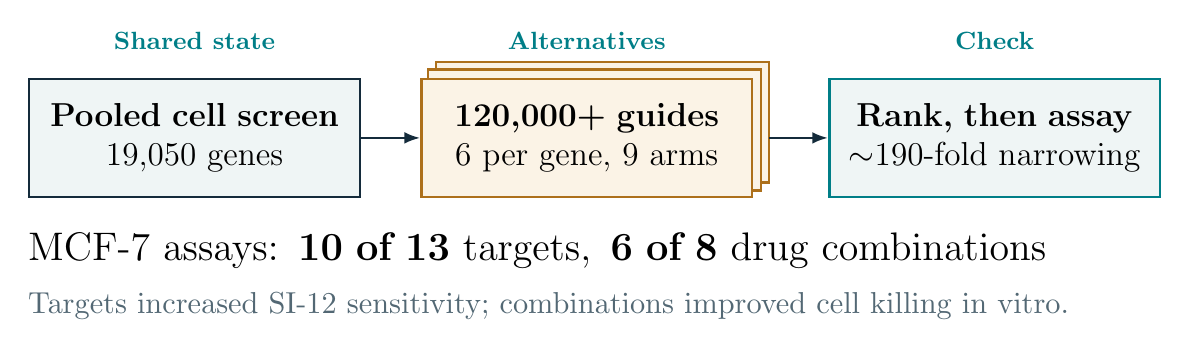
\begin{tikzpicture}[x=1cm,y=1cm,
  hd/.style={anchor=south,font=\fontsize{9.5}{11}\selectfont\bfseries,text=Teal},
  bx/.style={text width=3.9cm,inner xsep=.15cm,minimum height=1.5cm,font=\fontsize{11.5}{14}\selectfont},
  stack/.style={draw=Gold,fill=Sand,line width=.9pt},
  res/.style={anchor=north west,inner sep=0pt,text width=14.4cm,align=left,font=\fontsize{14.5}{17.5}\selectfont},
  ctx/.style={anchor=north west,inner sep=0pt,text width=14.4cm,align=left,font=\fontsize{10.5}{13}\selectfont,text=Muted},
  every node/.style={align=center}]
\useasboundingbox (0,.55) rectangle (14.4,-3.3);
\node[hd] at (2.12,.15) {Shared state};
\node[hd] at (7.10,.15) {Alternatives};
\node[hd] at (12.28,.15) {Check};
\node[state,bx] (s) at (2.12,-.85) {\textbf{Pooled cell screen}\\19,050 genes};
\node[candidate,bx] (a) at (7.10,-.85) {\textbf{120,000+ guides}\\6 per gene, 9 arms};
\begin{scope}[on background layer]
\draw[stack] ($(a.south west)+(.2,.2)$) rectangle ($(a.north east)+(.2,.2)$);
\draw[stack] ($(a.south west)+(.1,.1)$) rectangle ($(a.north east)+(.1,.1)$);
\end{scope}
\node[evidence,bx] (c) at (12.28,-.85) {\textbf{Rank, then assay}\\$\sim$190-fold narrowing};
\draw[flow] (s.east)--(a.west);
\draw[flow] ($(a.east)+(.2,0)$)--(c.west);
\node[res] at (0,-2.05) {MCF-7 assays:\enspace \textbf{10 of 13} targets,\enspace \textbf{6 of 8} drug combinations};
\node[ctx] at (0,-2.8) {Targets increased SI-12 sensitivity; combinations improved cell killing in vitro.};
\end{tikzpicture}
\claim{Six guides are six looks at one gene: count the gene once.\hspace{.8em}\hfill\exchip{COUNT ONCE}}
\sources{\href{https://doi.org/10.1038/s42003-021-01929-1}{Gilad, Eliaz et al., Communications Biology 4:399 (2021)}, Fig.~3. Ranking nominates candidates for validation.}
\qadetail{Count-once reading: guide effects are combined into one gene-level call, so the gene, not the guide, is the counted unit; DRACO keeps a gene only if at least four of its six guide effects agree with the mean direction, then ranks by the most extreme retained effect. Terrace and DRACO are distinct analyses of the same data, not independent evidence streams. 19,050 is the target-gene count; the library contains over 120,000 guide sequences including controls and other targets. Six guides per gene target different DNA sites. Three conditions (vehicle, SI-12, fulvestrant) with three biological replicate arms each give nine pooled arms. Cultures share the initial infected cell pool; the guide-variant and replicate structure is the fan-out analogy, without physical checkpoint copies. The approximately 190-fold narrowing is 19,050 / approximately 100 genes, not an exact unique-hit count. Eight targets with available inhibitors plus five further siRNA genes give 13 genetic follow-up targets, of which 10 increased sensitivity to SI-12; eight drug combinations were tested, of which six improved killing in MCF-7 cells (efficacy level at least 3). These are different assays and denominators. Viability points have at least four technical replicates and plots at least two independent experiments, distinct from the screen's three biological replicate arms. In-vitro results: no clinical effect, no proof every hit is on target. Schultz and Coelingh Bennink (Communications Biology 5:835, 2022) questioned several hits' target expression. The laboratory screen preceded computational ranking. A computational fork of analysis variants is a proposed use, not an experiment in this paper. The 2019 SI-2 study and this 2021 SI-12 screen are distinct projects. Full source: Gilad, Eliaz, Yu, Dean, Han, Qin, O'Malley and Lonard, Communications Biology 4, 399 (2021), DOI 10.1038/s42003-021-01929-1.}
% Transition: Repeated looks at one gene count once; the next example finds one family that looked like two.
\note{[1:05] Fourth, genomics, from work with my coauthors. The shared state is one pooled cell screen covering 19,050 genes. The alternatives are guides: six per gene, over a hundred twenty thousand, across nine pooled arms. Two ranking methods, one requiring four of six guides to agree, narrowed nineteen thousand genes to about one hundred. Here is the counting lesson. Six guides are six looks at one gene, not six discoveries, so the gene counts once, like a road on the map. Rule two. Then the check: focused assays in MCF-seven breast cancer cells. Ten of thirteen genetic targets increased sensitivity to SI-twelve; six of eight drug combinations improved killing. Different assays, different denominators, and laboratory results, not clinical ones. Next, one family that looked like two.}
\end{frame}

% Act 2 example: shared template for short/10--14 (same geometry; only text and rule chips change).
% Rule chip: gold, right-aligned on the claim line; names match the map columns on slides 3, 15 and 26.
\providecommand{\exchip}[1]{\tikz[baseline=(x.base)]\node[fill=Gold,text=white,rounded corners=1.5pt,inner xsep=2.6pt,inner ysep=1.7pt,font=\fontsize{7.6}{8.6}\selectfont\bfseries](x){#1};}
\begin{frame}[t]{\ev{\tagM}\surf{PHYSICS}With Ori Chamo, we connected two apparent branches of one orbit family.\strut}
\vspace{.15cm}
\noindent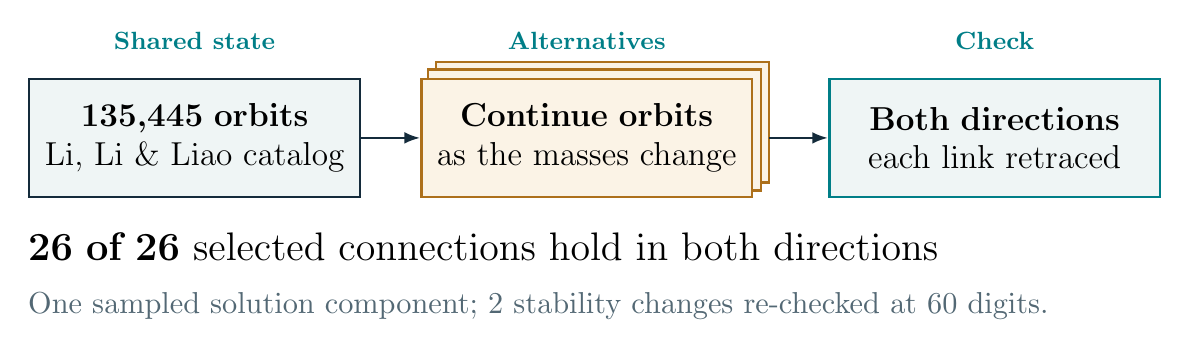
\begin{tikzpicture}[x=1cm,y=1cm,
  hd/.style={anchor=south,font=\fontsize{9.5}{11}\selectfont\bfseries,text=Teal},
  bx/.style={text width=3.9cm,inner xsep=.15cm,minimum height=1.5cm,font=\fontsize{11.5}{14}\selectfont},
  stack/.style={draw=Gold,fill=Sand,line width=.9pt},
  res/.style={anchor=north west,inner sep=0pt,text width=14.4cm,align=left,font=\fontsize{14.5}{17.5}\selectfont},
  ctx/.style={anchor=north west,inner sep=0pt,text width=14.4cm,align=left,font=\fontsize{10.5}{13}\selectfont,text=Muted},
  every node/.style={align=center}]
\useasboundingbox (0,.55) rectangle (14.4,-3.3);
\node[hd] at (2.12,.15) {Shared state};
\node[hd] at (7.10,.15) {Alternatives};
\node[hd] at (12.28,.15) {Check};
\node[state,bx] (s) at (2.12,-.85) {\textbf{135,445 orbits}\\Li, Li \& Liao catalog};
\node[candidate,bx] (a) at (7.10,-.85) {\textbf{Continue orbits}\\as the masses change};
\begin{scope}[on background layer]
\draw[stack] ($(a.south west)+(.2,.2)$) rectangle ($(a.north east)+(.2,.2)$);
\draw[stack] ($(a.south west)+(.1,.1)$) rectangle ($(a.north east)+(.1,.1)$);
\end{scope}
\node[evidence,bx] (c) at (12.28,-.85) {\textbf{Both directions}\\each link retraced};
\draw[flow] (s.east)--(a.west);
\draw[flow] ($(a.east)+(.2,0)$)--(c.west);
\node[res] at (0,-2.05) {\textbf{26 of 26} selected connections hold in both directions};
\node[ctx] at (0,-2.8) {One sampled solution component; 2 stability changes re-checked at 60 digits.};
\end{tikzpicture}
\claim{Two branches in a plot, one family in solution space.\hspace{.8em}\hfill\exchip{COUNT ONCE}}
\sources{With \textbf{Ori Chamo}. \href{https://ai.vixra.org/abs/2608.0069}{Chamo--Eliaz preprint (2026)}, not peer reviewed; \href{https://github.com/zozo123/threebody-closing-the-open}{Atlas numerical records}.}
\qadetail{Full source: Ori Chamo and Yossi Eliaz, Continuation geometry resolves apparent branch splitting in unequal-mass three-body orbits, ai.viXra:2608.0069v1 (2026); numerical records at https://github.com/zozo123/threebody-closing-the-open. The work is preliminary and not peer reviewed. The 135,445 entries originate in Li, Li and Liao's catalog, which described one family (2021); Stancevic, Vasiljevic and Dmitrasinovic (2023) interpreted the period/angular-momentum projection as two sets. We resolve the inference from projected separation to disconnected dynamics, without disproving the 2023 analysis on its own projected-coordinate terms. The 26 selected tests are five macroscopic bottlenecks, twenty large chart discontinuities and one long-range near-coincident projected pair; all succeed bidirectionally. This establishes connection within one sampled continuation component, not global completeness. Stability is separate from connectivity: two representative physical Floquet stability transitions have independent 60-digit Verner-integrator checks; not every catalog orbit was checked at that precision, and the 60-digit work is not the evidence for the 26 connections. Extra-Trees active learning proposes warm starts and is not the proof behind the 26 connections. An unresolved coarse mpmath RK4 cross-check was rejected as evidence. Numerical continuation changes a solution and corrects it; it is not physical forking. This is an evidence-admission example, not a sandbox-fork performance result.}
% Transition: Five fields, one loop; the synthesis names the three rules they share.
\note{[1:05] Fifth, physics, with Ori Chamo. The shared state is a catalog: Li, Li and Liao tabulated 135,445 periodic three-body orbits and described one family. A later analysis plotted the same catalog and saw two branches. Our alternatives are continuations: change the masses in small steps and correct each orbit so it keeps repeating. A connection counts only if it holds in both directions. All twenty-six selected connections did, so the links join one sampled solution component. The plot made one family look like two; count it once. Separately, two stability changes reproduced at sixty digits. This is a preprint, not peer reviewed, and not a completeness proof. Next, the three rules all five examples share.}
\end{frame}

% THE MAP, second of three uses (03, 15, 26). The \providecommand block below is copied verbatim from 03-promise.tex; keep the three identical.
% Arguments: #1 #2 #3 = column bodies (compute once, count once, publish once); #4 = extra TikZ.
\providecommand{\rulemap}[4]{%
\noindent\begin{tikzpicture}[x=1cm,y=1cm,
  rh/.style={evidence,text width=4.2cm,minimum height=.9cm,font=\fontsize{12}{14}\selectfont\bfseries,text=Teal},
  rs/.style={anchor=north,inner sep=0pt,font=\fontsize{10}{12}\selectfont,text=Muted},
  rb/.style={anchor=north,inner sep=0pt,text width=4.7cm,align=center,font=\fontsize{12}{14.5}\selectfont}]
\useasboundingbox (0,1.05) rectangle (14.4,-3.75);
\node[rh] (r1) at (2.3,0) {1\enspace COMPUTE ONCE};
\node[rh] (r2) at (7.2,0) {2\enspace COUNT ONCE};
\node[rh] (r3) at (12.1,0) {3\enspace PUBLISH ONCE};
\draw[flow] (r1)--(r2);\draw[flow] (r2)--(r3);
\draw[message] (r3.north)--++(0,.42)-|node[pos=.25,above,inner sep=1.5pt,font=\fontsize{9}{10}\selectfont,text=Teal]{continue} (r1.north);
\node[rs] at (2.3,-.62) {Runtime};
\node[rs] at (7.2,-.62) {Evidence};
\node[rs] at (12.1,-.62) {Acceptance};
\node[rb] at (2.3,-1.15) {#1};
\node[rb] at (7.2,-1.15) {#2};
\node[rb] at (12.1,-1.15) {#3};
#4
\end{tikzpicture}\par}
\begin{frame}[t]{\ev{\tagP}\surf{THREE RULES}Five fields, one loop, three rules.}
\vspace{.1cm}
\rulemap{\fontsize{11.5}{14}\selectfont Fuzzer child set up once\\[4pt]Start from the incumbent}
{\fontsize{11.5}{14}\selectfont Crashes deduplicated\\[4pt]Six guides, one gene\\[4pt]Two branches, one family}
{\fontsize{11.5}{14}\selectfont Evaluator: keep or revert\\[4pt]One patch must be chosen}{}
\claim{\centering\forktree\enspace Compute once. Count once. Publish once.}
\sources{The five previous examples, by the rule each one shows. None measures our integrated runtime.}
\qadetail{The map from slide 3, now filled with the examples. AFL++ persistent mode reuses one initialized child across many inputs (its documentation reports typical 10--20x speedups); it wins by not forking for every input, provided critical state resets. CyberGym is a separate study: the authors manually confirmed 22 unique zero-days from 56 crashes; crashes and confirmed vulnerabilities are different units. Autoresearch ran one attempt at a time, with sequential Git keep or revert against a fixed evaluator. SWE-bench Lite 15.9 to 56 percent is candidate coverage, not selected success; a selector must still pick one patch. Six guides per gene are repeated looks at one gene; the assays confirm with their own denominators. In the three-body work, a projection made one orbit family look like two branches; the 60-digit checks cover two representative stability transitions and are separate from connectivity; the Chamo preprint is not peer reviewed. These are published or co-authored results that share the pattern; none measures our integrated runtime, and our own factory runs were serial with nothing forked.}
\note{[0:50] Back to our map. Five fields, one loop. Each started from a shared state, ran alternatives, and needed a check. And each one taught a rule. Compute once: the fuzzer sets up its child once, and each research attempt starts from the incumbent commit. Count once: duplicate crashes, six guides for one gene, and two apparent branches that were one orbit family. Publish once: a fixed evaluator decides keep or revert, and a selector must still choose one patch. Compute once. Count once. Publish once. Now rule one, in the runtime: what does a fork actually reuse?}
\end{frame}

\setact{3}
\begin{frame}[t]{\ev{\tagM\,\tagP}\surf{COMPUTE ONCE}The next step decides which state to reuse.}
\vspace{-.15cm}
\begin{center}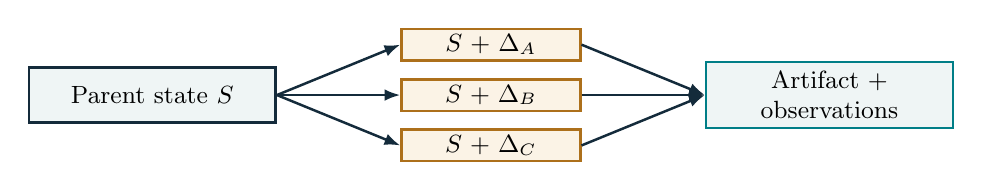
\begin{tikzpicture}[x=1cm,y=1cm,every node/.style={align=center,font=\fontsize{11}{13}\selectfont}]
\node[state,text width=2.9cm,minimum height=.7cm] (p) at (0,0) {Parent state $S$};
\foreach \k/\y in {A/.64,B/0,C/-.64}{\node[candidate,text width=2.2cm,minimum height=.4cm,inner sep=1pt] (c\k) at (4.3,\y) {$S+\Delta_\k$};\draw[flow] (p.east)--(c\k.west);}
\node[evidence,text width=2.9cm,minimum height=.7cm] (r) at (8.6,0) {Artifact +\\observations};
\foreach \k in {A,B,C}{\draw[flow] (c\k.east)--(r.west);}
\end{tikzpicture}\end{center}
\vspace{.02cm}
{\fontsize{11.5}{14}\selectfont\renewcommand{\arraystretch}{1.1}
\begin{tabularx}{\linewidth}{@{}L{4.3cm}L{5.0cm}Y@{}}
\toprule
\textcolor{Teal}{\textbf{Next step}} & \textcolor{Teal}{\textbf{Reuse by}} & \textcolor{Teal}{\textbf{Supplies}}\\
\midrule
Edit or rebuild & \textbf{Cache} & files, cached outputs\\
Continue a live run & \textbf{Restore} a checkpoint & the memory it keeps\\
Reuse an answer & \textbf{Replay} & the recorded response\\
\bottomrule
\end{tabularx}\par}
\vspace{.08cm}
{\fontsize{11.5}{14}\selectfont\tagM\enspace\textbf{Restore fan-out} on islo: 255/256 restore--run--capture calls succeeded.\par
\tagP\enspace Does live memory survive our restore? Untested until Gate~0 runs.\par}
\claim{Choose the cheapest mechanism that supplies what the next step reads.}
\sources{CRIU, gVisor, Firecracker, rr; SnowFlock (EuroSys 2009); DSec. Restores: \href{https://arxiv.org/abs/2607.09689}{arXiv:2607.09689v4}, Table~2.}
\qadetail{Fork semantics are backend-specific: filesystem clone, artifact cache, process fork, guest-memory restore and remote clone differ. A fork supplies several continuations from one captured parent with private writable state; fork identity is distinct from checkpoint identity and observation identity, and authority stays outside child-owned state. The three rows are the three ways to supply what the next step reads: rebuild from a cache (worktrees parallelize edits without preserving live processes), restore a checkpoint, or replay a record. The next slide prices a restore against a warm cache for a next step that reads only files, so a restore is compared with a warm cache, not with a cold start; a warm cache cannot continue a live run. Process checkpoints (CRIU, gVisor save/restore) and VM snapshots (Xen, SnowFlock, Firecracker) preserve only their declared state surfaces; the slide groups them without equating their supported state. Replay (rr, DSec) reuses a recorded response without reexecuting a remote service. Restore fan-out, measured: a named 141 MB islo snapshot, restore--run--capture round trips, 255 of 256 succeeded at concurrency 12, p50 6.87 s, p95 9.04 s, client-measured, teardown excluded from the percentiles (arXiv:2607.09689v4, Table 2). These are API round trips, not mechanism latency or a provider ranking, and they are separate from the factory runs, which used Docker sandboxes, serially, with nothing forked. A snapshot name does not establish memory semantics: memory preservation on this path is unverified, so the supported description is restore fan-out, not a memory fork; the Gate 0 RAM-only 128-bit nonce probe is preregistered and unrun. VM and process checkpoints can capture memory by design; the open question is only whether the path we restore keeps it. Network, time, randomness and remote model sessions need declared semantics; hosted-model weights, KV state and sampling stay outside the guest. The factory runs established files, dependencies and failed-test feedback, not a necessary live process; a running application at a reproduced failure is a hypothetical future workload. Editing loaded code may require reload or restart and invalidate the captured live state. SnowFlock: Lagar-Cavilla et al., EuroSys 2009, built on Xen.}
\note{[1:15] Rule one: compute once. Here is the fork again: a parent state S, and children that write only private changes. What S must hold depends on the next step. If it edits source or rebuilds, the first row is the cache from slide six: a worktree and build cache supply the files. If it continues a live run, we restore a process or VM checkpoint and get only the memory that mechanism supports. If it only needs an earlier answer, replay returns the recording. Restore fan-out on islo, our sandbox service: many restores of one named snapshot; two hundred fifty-five of two hundred fifty-six restore-run-capture calls succeeded. Whether live memory survives is untested until Gate zero, our first preregistered probe, runs. So choose the cheapest mechanism that supplies what the next step reads. When the next step reads only files, a restore and a warm cache both supply them.}
\end{frame}

\begin{frame}[t]{\ev{\tagA\,\tagO}\surf{COMPUTE ONCE}A restore pays only if it beats a warm cache.}
\begin{columns}[T,onlytextwidth]
\begin{column}{.43\textwidth}
{\fontsize{9.5}{11}\selectfont\color{Teal}\bfseries THE RULE\par}
\vspace{.2cm}
{\centering\fontsize{16}{19}\selectfont$(N-1)P > H+N(R+D)$\par}
\vspace{.3cm}
{\fontsize{11}{13.5}\selectfont\renewcommand{\arraystretch}{1.15}
\begin{tabularx}{\linewidth}{@{}L{1.05cm}Y@{}}
$N$ & alternative runs {\color{Muted}(8)}\\
$P$ & setup each run would repeat\\
$H$ & save the state once {\color{Muted}(2)}\\
$R+D$ & restart + private writes {\color{Muted}(1+3)}\\
\end{tabularx}\par}
\end{column}
\begin{column}{.53\textwidth}
{\fontsize{9.5}{11}\selectfont\bfseries{\color{Gold}AVOIDED SETUP}\enspace{\color{Muted}vs}\enspace{\color{Ink!60}OVERHEAD}\par}
\vspace{.1cm}
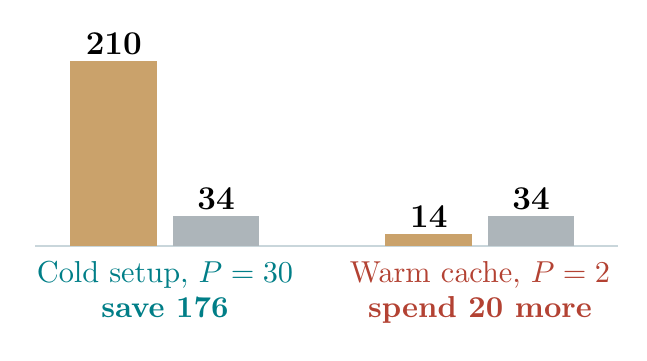
\begin{tikzpicture}[x=1cm,y=.0112cm,every node/.style={align=center,font=\fontsize{11}{13}\selectfont}]
\draw[Line,line width=.8pt] (0,0)--(7.4,0);
\fill[Gold!65] (.45,0) rectangle (1.55,210);
\fill[Ink!35] (1.75,0) rectangle (2.85,34);
\fill[Gold!65] (4.45,0) rectangle (5.55,14);
\fill[Ink!35] (5.75,0) rectangle (6.85,34);
\foreach \x/\v in {1.0/210,2.3/34,5.0/14,6.3/34}{\node[above,inner sep=2pt,font=\fontsize{11.5}{13}\selectfont\bfseries] at (\x,\v) {\v};}
\node[below,text=Teal] at (1.65,-6) {Cold setup, $P=30$\\\textbf{save 176}};
\node[below,text=Rust] at (5.65,-6) {Warm cache, $P=2$\\\textbf{spend 20 more}};
\end{tikzpicture}
\end{column}
\end{columns}
\vspace{.05cm}
{\fontsize{11}{13.5}\selectfont\color{Muted}Fastest public start: \textbf{73~ms} median to a first command, so $P$ must be real preparation.\par}
\claim{Price a restore against a warm cache, not a cold start.}
\sources{Illustrative additive model, resource-seconds. Start: \href{https://www.computesdk.com/benchmarks/sandboxes/burst-tti}{ComputeSDK Burst TTI} (Isorun median), 2 October 2026.}
\qadetail{The rule is an additive total-resource model, not measured elapsed time: work common to both alternatives cancels; D is incremental divergence overhead including copy-on-write; P must be reusable preparation, not merely sandbox setup. Batch elapsed time also depends on critical paths and contention. Worked illustration: N8, H2, R1, D3 give overhead 2+8(1+3)=34 resource-seconds; at a cold P30 reuse avoids (N-1)P=7x30=210 and saves 176; at a warm-cache P2 it avoids 14 and loses 20. These are sample calculations, not measured backend performance. Restoring saved state and rebuilding with a warm cache are both reuse; the comparison is between them, and a warm cache cannot be credited for a continuation it cannot supply. The comparison must reach equivalent usable state. The Tokio cache endpoints (about 46 s fresh, 13 s restored build files, 3 s already warm; author-reported, tokio issue 8200) appear earlier as artifact-cache timings, not fork timings. Starts: ComputeSDK Burst TTI (raw results SHA 24922f27408279200074cbc8773cbda9a4aa4785): create through first successful command at client concurrency 100, Isorun median 72.77 ms, p95 78.29 ms, 100/100. Our paper also recorded one provider's create path (Tensorlake, default environment, requested concurrency 8, 256/256 succeeded, median 3.44 s, p95 9.00 s, client API round trip, teardown excluded; arXiv:2607.09689v4, Table 2). That is not our platform. Creation versus time to first command and concurrency 8 versus 100 are different endpoints and protocols; do not divide one by the other. Jitsu (Madhavapeddy et al., NSDI 2015) and LightVM (Manco et al., SOSP 2017, NEC Labs) also illustrate cheap fresh starts. Latency form, which H1 tests: with the snapshot already taken, H is off the critical path and the N cells run in parallel, so restore wins makespan when R + D < P_warm; N enters only through contention, which is why H1 varies N = 3, 6, 12. The slide's resource form grows with N. The measured 6.87 s p50 (arXiv:2607.09689v4, Table 2) is a client restore--run--capture round trip, an upper bound that includes the run, not R itself; the R = 1 illustration is not a measured value. We do not claim that a fork is faster than a good build cache; the preregistered restore-versus-warm-cache experiment has not started.}
\note{[1:20] A question for you. You have a saved snapshot and a warm build cache. Restore the snapshot, or rebuild with the cache: which wins? With N alternative runs, each would repeat a setup cost, P; preparing once avoids N minus one copies. Against that we pay H to save the state once, and per child, R to restart it and D to keep its writes private. Take eight runs, H of two, R of one, D of three: thirty-four resource-seconds of overhead. With a cold setup of thirty, restoring avoids two hundred ten and saves a hundred seventy-six. With a warm cache, setup drops to two: restoring avoids only fourteen and costs twenty more. The warm cache wins: never build the same thing twice. Starts are cheap: the fastest provider in a public benchmark reached a first command in seventy-three milliseconds, so P must be real preparation. But even a winning restore cannot undo everything.}
\end{frame}

\begin{frame}[t]{\ev{\tagM\,\tagP}\surf{COMPUTE ONCE}A restore cannot undo remote effects, and a fork must not hold the right to publish.}
\vspace{-.05cm}
\begin{center}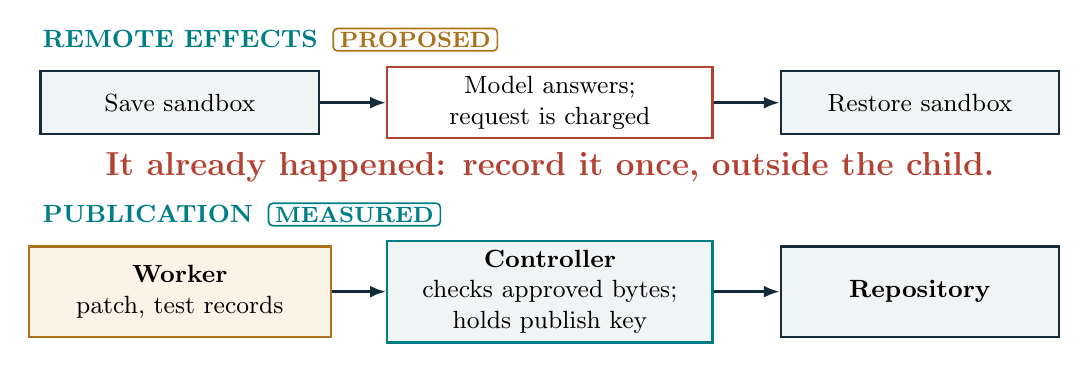
\begin{tikzpicture}[x=1cm,y=1cm,every node/.style={align=center,font=\fontsize{11.5}{14}\selectfont},
  head/.style={anchor=west,inner sep=0pt,font=\fontsize{9.5}{11}\selectfont\bfseries}]
\node[head,text=Teal] at (-1.75,.8) {REMOTE EFFECTS\enspace\tagP};
\node[state,text width=3.3cm,minimum height=.8cm] (a) at (0,0) {Save sandbox};
\node[bad,text width=3.9cm,minimum height=.8cm] (b) at (4.7,0) {Model answers;\\request is charged};
\node[state,text width=3.3cm,minimum height=.8cm] (c) at (9.4,0) {Restore sandbox};
\draw[flow] (a)--(b);\draw[flow] (b)--(c);
\node[text=Rust,font=\fontsize{12}{14.5}\selectfont\bfseries] at (4.7,-.82) {It already happened: record it once, outside the child.};
\node[head,text=Teal] at (-1.75,-1.42) {PUBLICATION\enspace\tagM};
\node[candidate,text width=3.6cm,minimum height=1.15cm] (w) at (0,-2.4) {\textbf{Worker}\\patch, test records};
\node[evidence,text width=3.9cm,minimum height=1.15cm] (k) at (4.7,-2.4) {\textbf{Controller}\\checks approved bytes;\\holds publish key};
\node[state,text width=3.3cm,minimum height=1.15cm] (r) at (9.4,-2.4) {\textbf{Repository}};
\draw[flow] (w)--(k);\draw[flow] (k)--(r);
\end{tikzpicture}\end{center}
\claim{Record effects once. Keep the publish key outside every fork.}
\sources{Output commit: Speculator, external synchrony, Remus. Effect journal: proposed; publish path: our factory runs.}
\qadetail{Restoring state cannot unsend a model or tool request, refund its cost or reverse a completed remote action; staging a patch keeps local bytes, while publication still needs a separate gate. An effect cannot be computed once by restoring; it can only be recorded once. Speculator, external synchrony and Remus are precedents for delaying output; DSec replays cached command results on resumption. A general effect journal is proposed, not built: stage effects where possible, reconcile uncertain outcomes, and use idempotency keys when the remote service supports them; an uncertain remote action cannot be blindly retried. Export the patch, inputs and receipts before every teardown, including refusal (motivated by SELFHOST-3). MEASURED scope: the factory runs (Docker Sandboxes via Airflow, serial, nothing forked) exercised one controller-mediated publication path with sha256-bound approval; they did not intercept every external effect. DESIGN scope: fresh clone authority, host authentication and authorization of each child outside copied guest state, revocable authorization and epoch fences are proposed. A fork copies every credential or capability in the guest: a microVM can contain a still-valid bearer token, and kernel isolation does not make that token harmless; so the publishing credential must never be placed in the guest. Guest-supplied generation strings are copied and cannot authenticate a clone, and fresh identity alone does not confer authority. Egress policy is distinct from withholding publication credentials. Siblings restored from one snapshot share every guest value: idempotency keys, userspace RNG state, boot_id, machine-id, MAC. A copied key would let a service merge N alternatives into one request; cloned userspace RNG can repeat nonces (Ristenpart and Yilek, NDSS 2010). VMGenID can reseed the kernel; userspace RNG treatment is application-dependent. H1 records boot_id, machine-id, IP/MAC, guest-minus-host clock and a userspace random value per cell (PREREGISTRATION.md, Phase A). Output-commit precedents: Speculator (Nightingale, Chen and Flinn, SOSP 2005), external synchrony (Nightingale et al., OSDI 2006), Remus (Cully et al., NSDI 2008). Capability systems that bound what a credential can do: Capsicum, CHERI.}
\note{[1:15] First, remote effects. Save a sandbox, call a hosted model, then restore. The sandbox is back before the call, but the model has already answered and charged us. Restoring cannot rewind another service, so an effect cannot be computed once by restoring; it must be recorded once. Our proposed design records the outcome outside the sandbox, reconciles anything uncertain, and retries with an idempotency key that the controller mints for each child, so a fork never copies it. Second, recall the Twistlock lesson: a sandbox is a policy boundary. A fork copies every credential inside it, so the right to publish must never be inside. A worker returns a patch with its test records. The controller checks that approval names those exact bytes, and only the controller holds the publish key. Our factory runs exercised that separation. What should each child hand it?}
\end{frame}

\setact{4}
\begin{frame}[t]{\ev{\tagM\,\tagP}\surf{COUNT ONCE}A receipt is evidence's cache entry, written outside the child.}
\vspace{.2cm}
\begin{center}
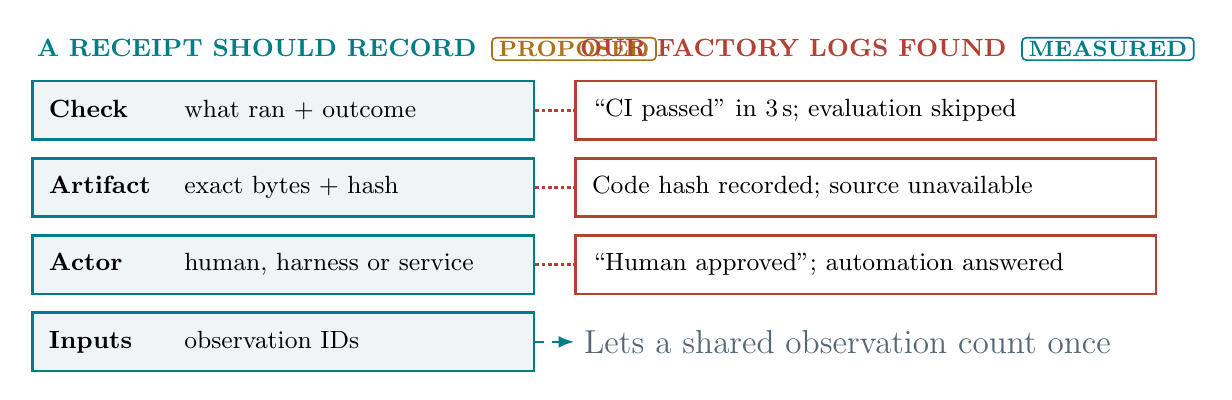
\begin{tikzpicture}[x=1cm,y=1cm,every node/.style={font=\fontsize{11.5}{14}\selectfont},
  field/.style={evidence,anchor=west,text width=5.95cm,minimum height=.74cm,align=left,inner xsep=6pt},
  found/.style={bad,anchor=west,text width=6.95cm,minimum height=.74cm,align=left,inner xsep=6pt},
  head/.style={anchor=west,font=\fontsize{9}{10}\selectfont\bfseries}]
\node[head,text=Teal] at (-.05,.78) {A RECEIPT SHOULD RECORD\enspace\tagP};
\node[head,text=Rust] at (6.85,.78) {OUR FACTORY LOGS FOUND\enspace\tagM};
\node[field] (f1) at (0,0)     {\makebox[1.72cm][l]{\textbf{Check}}what ran + outcome};
\node[field] (f2) at (0,-.98) {\makebox[1.72cm][l]{\textbf{Artifact}}exact bytes + hash};
\node[field] (f3) at (0,-1.96)  {\makebox[1.72cm][l]{\textbf{Actor}}human, harness or service};
\node[field] (f4) at (0,-2.94) {\makebox[1.72cm][l]{\textbf{Inputs}}observation IDs};
\node[found] (r1) at (6.9,0)     {``CI passed'' in 3\,s; evaluation skipped};
\node[found] (r2) at (6.9,-.98) {Code hash recorded; source unavailable};
\node[found] (r3) at (6.9,-1.96)  {``Human approved''; automation answered};
\node[anchor=west,text=Muted,font=\fontsize{11.5}{14}\selectfont] (r4) at (6.9,-2.94) {Lets a shared observation count once};
\foreach \i in {1,2,3}{\draw[relation] (f\i.east)--(r\i.west);}
\draw[message] (f4.east)--(r4.west);
\end{tikzpicture}
\end{center}
\sources{Three audit findings from our factory records (SELFHOST-2 approvals and adapter; CI, 28 September 2026). Typed receipt fields are proposed. Related provenance: PASS, CamFlow, in-toto.}

\qadetail{Who writes it: in the proposed design the harness or controller writes the receipt, outside the child's trust boundary; a report written by the child about itself is only a claim. These are reported own audit findings, not three fork-induced errors; the factory runs used Docker sandboxes, ran serially and forked nothing. The evals-islo Actions job (run 36423283572) passed in about three seconds while its real evaluation step was skipped because a key was absent. Approvals recorded mode human and actor admin although the harness answered the intent and plan gates; this is an actor/event labeling issue and does not mean the harness performed the human review. A local adapter shim outside Git had a recorded digest but no recoverable source in the repository: a code hash identifies bytes; it does not store them. Cache-entry analogy: a receipt is written after execution and carries the outcome and actor, so it is an action-cache entry (key plus result), not a key alone. As in a remote-execution ActionResult, which also records the worker, the key fields (check, artifact hash, input IDs) make the same evidence recognisable, so it counts once; a hash proves identity, not correctness. Proposed typed states are executed, skipped and failed; proposed actors are human, harness and service. Authenticity alone does not establish semantic accuracy. Audit inspects records; replay requires retrievable adapter bytes and recorded external responses; fresh hosted-model calls create a fresh run. Identity checks and external recording address integrity; they do not establish behavioral coverage or calibration. Related: PASS, CamFlow, in-toto, rr, DSec.}
\note{[1:15] Rule two: count once. Parallel trials share inputs and errors, so we need a record of what each trial did. That record is a receipt. It works like a cache entry: the key is what ran, on which bytes, from which inputs; the value is the outcome and who reported it. The bytes are named by the hash from slide six. In our design the factory's harness, not the agent, writes it, outside the child; a child's report about itself is only a claim. Our factory logs show why each field matters. A CI job passed in three seconds; its evaluation had been skipped. A code hash was recorded, but the helper's source was unavailable. A hash is a fingerprint, not a backup. An approval was labelled human, but automation answered it. The last field, inputs, is what lets us count a shared observation once. Next: combining receipts.}
\end{frame}

\begin{frame}[t]{\ev{\tagA\,\tagP}\surf{COUNT ONCE}Each fan-in operation needs its own check.}
\vspace{.1cm}
\begin{center}
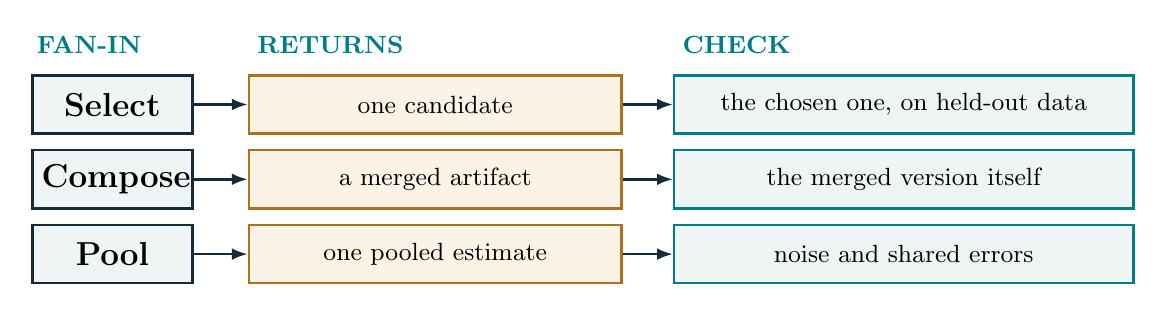
\begin{tikzpicture}[x=1cm,y=1cm,every node/.style={font=\fontsize{11.5}{14}\selectfont},
  op/.style={state,anchor=west,text width=1.8cm,minimum height=.74cm,font=\fontsize{11.5}{14}\selectfont\bfseries},
  ret/.style={candidate,anchor=west,text width=4.5cm,minimum height=.74cm},
  chk/.style={evidence,anchor=west,text width=5.6cm,minimum height=.74cm},
  head/.style={anchor=west,font=\fontsize{9}{10}\selectfont\bfseries,text=Teal}]
\node[head] at (-.05,.75) {FAN-IN};
\node[head] at (2.75,.75) {RETURNS};
\node[head] at (8.15,.75) {CHECK};
\foreach \y/\o/\r/\c in {0/Select/one candidate/{the chosen one, on held-out data},-.95/Compose/a merged artifact/{the merged version itself},-1.9/Pool/one pooled estimate/{noise and shared errors}}{
  \node[op] (o) at (0,\y) {\o};
  \node[ret] (r) at (2.75,\y) {\r};
  \node[chk] (c) at (8.15,\y) {\c};
  \draw[flow] (o)--(r);\draw[flow] (r)--(c);
}
\end{tikzpicture}
\end{center}
\vspace{.3cm}
{\centering\fontsize{11.5}{14}\selectfont\textbf{Why test the merge?}\enspace Each change starts a 1\,GB worker; the server has 2\,GB.\par}
\begin{center}
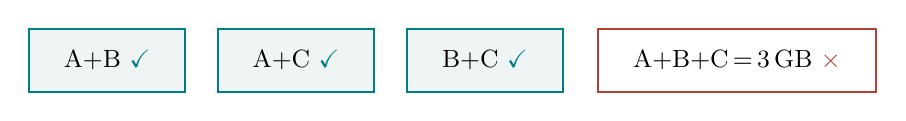
\begin{tikzpicture}[x=1cm,y=1cm,every node/.style={font=\fontsize{11.5}{14}\selectfont,minimum height=.6cm,align=center}]
\node[evidence,text width=1.75cm] at (0,0) {A+B \yes};
\node[evidence,text width=1.75cm] at (2.4,0) {A+C \yes};
\node[evidence,text width=1.75cm] at (4.8,0) {B+C \yes};
\node[bad,text width=3.3cm] at (8.0,0) {A+B+C\,=\,3\,GB \no};
\end{tikzpicture}
\end{center}
\sources{Illustrative capacity example, not a recorded incident. Union and intersection are further fan-in rules (Q\&A).}

\qadetail{The three rows describe decision semantics, not three implemented end-to-end systems. Selection needs a fixed evaluator over eligible candidates; argmax returns the candidate while max returns only its score, so keep candidate identity and a deterministic tie rule. Selection is adaptive, so the chosen candidate needs fresh evaluation for generalization; a deterministic regression check can still establish its asserted behavior. Coverage is not selected success (the patch-selector point from the software-engineering example). Code merge is a partial operation on edits from the same base: it may be undefined for conflicting edits or depend on conflict resolution, and it is checked on its final output. No universal associative or commutative code-merge law is claimed. The 1 GB example is illustrative and exact, not a recorded software incident: with U=1 for pass, Gamma_ij=U({i,j})-U({i})-U({j})+U(empty) gives zero pair interactions and a failing triple. Pooling requires one common target, calibrated information and a dependence model; it cannot combine different artifacts simply because each returns a number. The full menu also has union for disjoint shards (check coverage and duplicates), intersection for common findings (agreement can reflect a shared error) and a weighted mean with weights summing to one. ReLU is a pointwise transform, not a fan-in rule.}
\note{[1:10] Once trials return receipts, we combine them. That step is fan-in, and it is not one operation. If the trials tried different ideas, we select one candidate; that is the patch selector from the software example. Selection is itself a search, so we check the winner again, on held-out data. If the trials edited different parts of a program, we compose their edits, and the merged version needs its own test. A made-up example: each of three changes starts a one-gigabyte worker, and the server has two gigabytes. Each change alone fits. Every pair fits. All three together need three gigabytes and fail. No pair test covered that state. Finally, if the trials estimated the same quantity, we pool them, and the weights must account for errors they share. Next: what that sharing costs.}
\end{frame}

\begin{frame}[t]{\ev{\tagA\,\tagB}\surf{COUNT ONCE}Overlapping trials add less than their count.}
\vspace{.05cm}
\begin{center}
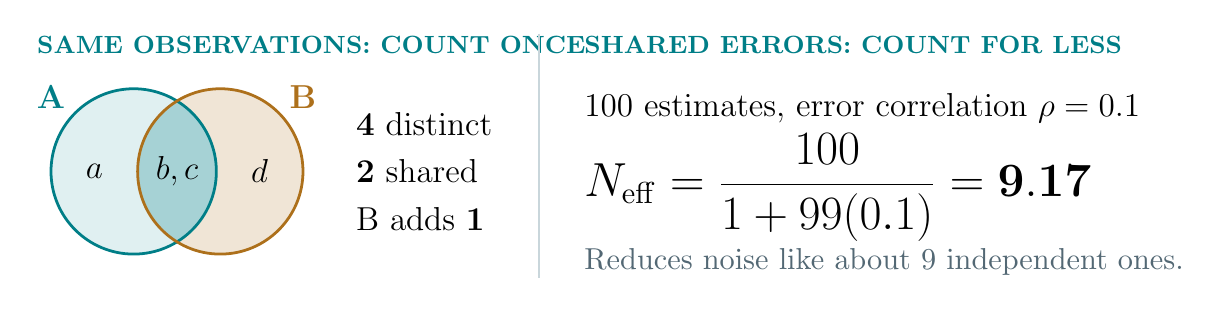
\begin{tikzpicture}[x=1cm,y=1cm,every node/.style={font=\fontsize{11.5}{14}\selectfont},
  head/.style={anchor=west,font=\fontsize{9}{10}\selectfont\bfseries,text=Teal}]
\node[head] at (-.05,1.8) {SAME OBSERVATIONS: COUNT ONCE};
\node[head] at (6.9,1.8) {SHARED ERRORS: COUNT FOR LESS};
\draw[Line,line width=.6pt] (6.45,1.95)--(6.45,-1.15);
% Left: two trials that return overlapping observation IDs.
\fill[Teal!12](1.3,.2)circle(1.05);\fill[Gold!18](2.4,.2)circle(1.05);
\begin{scope}\clip(1.3,.2)circle(1.05);\fill[Teal!35](2.4,.2)circle(1.05);\end{scope}
\draw[Teal,line width=1pt](1.3,.2)circle(1.05);\draw[Gold,line width=1pt](2.4,.2)circle(1.05);
\node[font=\fontsize{12}{14}\selectfont\bfseries,text=Teal] at (.25,1.15) {A};
\node[font=\fontsize{12}{14}\selectfont\bfseries,text=Gold] at (3.45,1.15) {B};
\node[font=\fontsize{12.5}{15}\selectfont] at (.8,.2) {$a$};
\node[font=\fontsize{12.5}{15}\selectfont] at (1.85,.2) {$b,c$};
\node[font=\fontsize{12.5}{15}\selectfont] at (2.9,.2) {$d$};
\node[anchor=west,align=left,font=\fontsize{12}{17}\selectfont] at (4.0,.2) {\textbf{4} distinct\\\textbf{2} shared\\B adds \textbf{1}};
% Right: correlated errors shrink the effective count.
\node[anchor=west] at (6.9,1.0) {100 estimates, error correlation $\rho=0.1$};
\node[anchor=west,font=\fontsize{16}{19}\selectfont] at (6.9,.0) {$N_{\rm eff}=\dfrac{100}{1+99(0.1)}=\mathbf{9.17}$};
\node[anchor=west,text=Muted,font=\fontsize{11}{13}\selectfont] at (6.9,-.95) {Reduces noise like about 9 independent ones.};
\end{tikzpicture}
\end{center}
{\centering\fontsize{11}{13}\selectfont\color{Muted}Seen before: one road, many drives (Roadbook); one gene, six guides (screen).\par}
\vspace{.12cm}
{\color{Line}\rule{\linewidth}{.6pt}}\par
\vspace{.08cm}
{\fontsize{11}{15}\selectfont
\tagB\enspace Our reducer rejects duplicate observation IDs and carries lineage.\par
{\color{Gold}\bfseries Proposed:}\enspace covariance-aware weights; refuse unsupported precision claims.\par}
\sources{Illustrative: exact set IDs; equal noise, common pairwise correlation. \href{https://github.com/zozo123/boltzmann-mapreduce}{Reference reducer}; \href{https://arxiv.org/html/2607.09689v4}{arXiv:2607.09689v4}.}

\qadetail{The set diagram counts exact illustrative observation IDs; circle areas do not represent entropy or Fisher information. Deduplicating declared IDs does not measure correlation between different items; distinct IDs do not authenticate observations or prove independence, and a copied receipt remains the same observation. The 100-estimate example assumes equal marginal noise sigma and a common pairwise correlation, with the signal held fixed: Var = sigma^2[rho+(1-rho)/N], so noise is 0.10 sigma independent versus 0.33 sigma at rho=0.1, and the signal-to-noise gain is 10x versus 3.03x. N_eff is variance-equivalent precision for a mean, not a count of independent units, not a probability of correctness, and it does not remove shared bias. Candidate search needs a different joint quantity (the all-wrong probability). The Roadbook and guide callbacks are analogies: matched drives of one road and six guides per gene are repeated looks at one target, not forks or measured correlations. The built Gaussian/Wald reference reducer adds natural-parameter summaries associatively under an independence/common-target model; a declared duplicate evidence ID raises; lineage is transported but not yet consumed. It does not abstain. Proposed: covariance-aware weights w = Sigma^-1 1 / (1^T Sigma^-1 1) (best linear unbiased under known positive-definite covariance; Valassi and Chierici 2014), with covariance from justified calibration rather than worker declarations; weights can be negative and common bias does not average away. Also proposed: abstention when dependence is unknown, trusted evidence identity and controller-derived information. Source: Eliaz, arXiv:2607.09689v4.}
\note{[1:10] Overlap shows up in two ways. First, trials can return the same observations. Trial A returns a, b and c; trial B returns b, c and d. That is four distinct observations, not six, so B adds only d. Count each observation once, the way the Roadbook counts each road once. Second, different observations can still share errors, like six guides aimed at one gene. Take a hundred equally noisy estimates whose errors have pairwise correlation point one. Their average reduces noise like about nine independent estimates, not a hundred. Today, our reducer rejects a duplicate observation ID and keeps each result's source history. It does not yet use that history to set weights; covariance-aware weights, and refusing a precision claim when dependence is unknown, are proposed. Next: a worker that overstates its own precision.}
\end{frame}

\begin{frame}[t]{\ev{\tagM}\surf{COUNT ONCE}A worker that overstates its precision can take over the average.}
\vspace{.05cm}
\begin{columns}[T,totalwidth=\linewidth]
\begin{column}{.47\linewidth}
\vspace{.1cm}
{\fontsize{18}{22}\selectfont$\displaystyle\hat\mu=\frac{\sum_i p_i\,x_i}{\sum_i p_i}$\par}
\vspace{.3cm}
{\fontsize{12.5}{16}\selectfont$p_i$: \textbf{reported} precision (1\,/\,variance).\\More precision, more weight.\par}
\vspace{.3cm}
{\fontsize{11.5}{14}\selectfont\color{Muted}Synthetic: one worker, 2,000 points\\near~17, information per point $\times50$.\par}
\end{column}
\begin{column}{.51\linewidth}
\centering
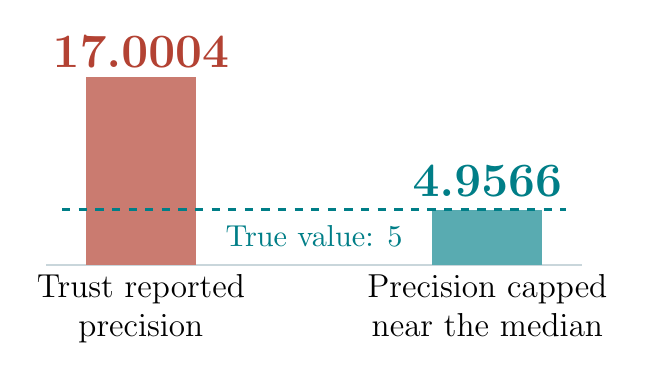
\begin{tikzpicture}[x=1cm,y=.14cm,every node/.style={align=center,font=\fontsize{11.5}{14}\selectfont}]
\draw[Line,line width=.6pt](-.2,0)--(6.6,0);
\fill[Rust!70](.3,0)rectangle(1.7,17.0004);\fill[Teal!65](4.7,0)rectangle(6.1,4.9566);
\draw[Teal,dashed,line width=1pt](0,5)--(6.4,5);
\node[anchor=north,text=Teal,font=\fontsize{11}{13}\selectfont] at (3.2,4.5) {True value: 5};
\node[above,font=\fontsize{16}{19}\selectfont\bfseries,text=Rust]at(1.0,17.0004){17.0004};
\node[anchor=south,font=\fontsize{16}{19}\selectfont\bfseries,text=Teal]at(5.4,5.3){4.9566};
\node[below]at(1.0,0){Trust reported\\precision};\node[below]at(5.4,0){Precision capped\\near the median};
\end{tikzpicture}
\end{column}
\end{columns}
\claim{Check outside the child, including its error bars.}
\sources{\href{https://github.com/zozo123/boltzmann-mapreduce/blob/main/demo.py}{Reference demo}: one synthetic stress case, not a Byzantine guarantee; the rule needs trusted precision.}

\qadetail{Verified primary demo.py lines 90--93 sets true_theta 5.0; lines 151--165 set liar_theta = true_theta + 12, SD .02, count 2000, multiplier 50. This target is distinct from the full-sample 4.9450 in the separate islo integration trace. The 2000-point shard returns a distant estimate and reports fiftyfold information per point. Unprotected pooling yields 17.0004; the stress heuristic yields 4.9566. Sample count alone cannot detect this claim. The heuristic illustrates one stress case, not a Byzantine guarantee. The heuristic (bmr/core.py byzantine_clip, kappa 3) caps total reported precision at the cross-worker median plus 3 MAD and down-weights by 1e-6 any estimate more than 3 MAD from the median estimate. It compares workers with each other, so it assumes an honest majority and would also suppress a lone correct worker; trusted recomputation outside the child is the proposed check. Trusted recomputation under the numerical model can validate information; agent scores need a separately validated error model. These extensions are proposed. An external recorder alone does not establish statistical calibration. Calibrated information and a shared parameter are prerequisites; no general agent score improvement is inferred. Five shard sizes are 60, 120, 400, 2000, 5000. Mean norm gap to centralized MLE over eight fixed seeds is .0083 plus/minus .0042 for information pooling and .177 plus/minus .090 for equal averaging; these are SD, not confidence intervals. Sample-size weighting was not compared. Separate four-worker islo integration trace from a 141 MB snapshot pooled synthetic mean 4.9422 versus full-sample 4.9450, gap .0028, in 6.70 s client restore--run--capture. This tests aggregation and an exercised integration path, not agent accuracy or dependence correction.}
\note{[1:00] A weighted average multiplies each estimate by its precision, one over its variance, and divides by the total. A worker that claims little uncertainty gets a large weight. In our synthetic test the true value is five. One worker sends two thousand tightly packed points near seventeen and inflates its information per point fiftyfold. Counting points would not catch it. Trusting the reported precision, the average is seventeen point zero zero zero four: one worker took over. Capping each worker's precision near the peer median returns four point nine five six six. One synthetic case, not a Byzantine guarantee. As with receipts: check outside the child, including its error bars. Even an honest count is not yet permission to publish.}
\end{frame}

\setact{5}
\begin{frame}[t]{\ev{\tagM\,\tagP}\surf{PUBLISH ONCE}Accept only bytes whose promise was tested.}
\vspace{-.1cm}
\begin{center}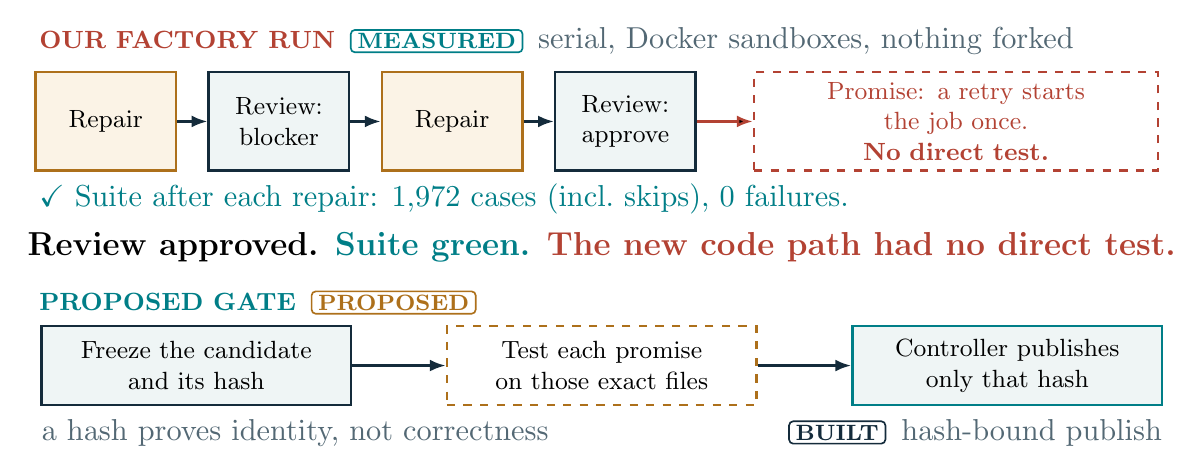
\begin{tikzpicture}[x=1cm,y=1cm,every node/.style={align=center,font=\fontsize{11}{13.5}\selectfont},
  head/.style={anchor=west,inner sep=0pt,font=\fontsize{9.5}{11}\selectfont\bfseries}]
\node[head,text=Rust] at (0,1.02) {OUR FACTORY RUN\enspace\tagM\enspace{\mdseries\fontsize{10.5}{12}\selectfont\color{Muted}serial, Docker sandboxes, nothing forked}};
\node[candidate,text width=1.55cm,minimum height=1.25cm] (r1) at (.85,0) {Repair};
\node[state,text width=1.55cm,minimum height=1.25cm] (v1) at (3.05,0) {Review:\\blocker};
\node[candidate,text width=1.55cm,minimum height=1.25cm] (r2) at (5.25,0) {Repair};
\node[state,text width=1.55cm,minimum height=1.25cm] (v2) at (7.45,0) {Review:\\approve};
\node[missing,text width=4.9cm,minimum height=1.25cm] (m) at (11.65,0) {Promise: a retry starts\\the job once.\\\textbf{No direct test.}};
\draw[flow] (r1)--(v1);\draw[flow] (v1)--(r2);\draw[flow] (r2)--(v2);\draw[denied] (v2)--(m);
\node[anchor=west,inner sep=0pt,text=Teal,font=\fontsize{11}{13}\selectfont] at (0,-.98) {\yes\ Suite after each repair: 1,972 cases (incl.\ skips), 0 failures.};
\node[inner sep=0pt,font=\fontsize{12.5}{15}\selectfont\bfseries] at (7.15,-1.6) {Review approved. \textcolor{Teal}{Suite green.} \textcolor{Rust}{The new code path had no direct test.}};
\node[head,text=Teal] at (0,-2.3) {PROPOSED GATE\enspace\tagP};
\node[state,text width=3.7cm,minimum height=1cm] (g1) at (2.0,-3.1) {Freeze the candidate\\and its hash};
\node[proposed,text width=3.7cm,minimum height=1cm] (g2) at (7.15,-3.1) {Test each promise\\on those exact files};
\node[evidence,text width=3.7cm,minimum height=1cm] (g3) at (12.3,-3.1) {Controller publishes\\ only that hash};
\draw[flow] (g1)--(g2);\draw[flow] (g2)--(g3);
\node[labeltext,anchor=west,inner sep=0pt,font=\fontsize{11}{13}\selectfont] at (.03,-3.95) {a hash proves identity, not correctness};
\node[labeltext,anchor=east,inner sep=0pt,font=\fontsize{11}{13}\selectfont] at (14.27,-3.95) {\tagB\enspace hash-bound publish};
\end{tikzpicture}\end{center}
\sources{SELFHOST-2, 27 September 2026: PR \#2351, zozo123/ariflow-swfactory; merged 3 October 2026 after I reverted the out-of-scope, untested path outside the factory. Gate: proposed; hash-bound publish: built.}
\qadetail{MEASURED scope: SELFHOST-2 (27 Sep 2026; PR \#2351 of zozo123/ariflow-swfactory, docs/factory/SELFHOST-2/) ran serially on Docker sandboxes (toolset SbxCommaPolicyBackend), not on islo; nothing forked, and the work graph recorded serial-fallback-missing-fork. The harness answered the intent and plan gates; approvals.json records mode human, actor admin. All four agent steps used the same hosted model. Repair 1 had no shell tool, did not run the tests, and changed backend/service.py, outside the six approved files. Review 1 returned request-changes with a blocker requesting deterministic tests. Repair 2 reported that tests/ were protected and refactored the helper; no blocked edit attempt is recorded and the test-edit hook never fired (15 edits, all allowed). Review 2 approved, kept the out-of-plan file major and downgraded untested to minor. The harness ran the full suite after each repair, on the candidate bytes: 1,972 cases including skips and zero failures, not 1,972 passing tests. So the failure was not that the bytes changed after the check; it was that no test exercised the new promise. The retry example abbreviates a specific same-work-order CellBusy-adoption path; it does not claim a general or proven exactly-once protocol. The new code path lands with no test in the diff; its only coverage is the race, reached only when the interleaving happens to lose an activation, which is not a deterministic test of that path. The missing test is an unresolved acceptance obligation, not proof that the patch was wrong. Review approved refers to review 2's approve verdict; the gap lay in the check, not in a gamed result: the harness, not an agent, ran the suite and recorded zero failures, and review 2 itself recorded that the path lands with no test. Merge: I reverted the out-of-plan service.py change outside the factory, as out of plan scope (commit 561c268c, 27 Sep, Revert the fix loop's out-of-scope Cell-ownership change). That removed the untested CellBusy-adoption path, and PR \#2351 then merged on 3 October 2026. The merge was my decision, not the factory's acceptance, and the untested path is not in the merged diff: a person removed the path the proposed gate would have refused. DESIGN scope: the gate is proposed and builds on the built sha256-bound publication check. The required test forces CellBusy with an active workspace owned by another attempt of the same job, holds the current dispatch authorization and asserts one backend dispatch; if no test exercises a promise the change makes, the gate refuses. Promises come from the approved plan and from review findings; a change outside the plan's files needs explicit scope authorization plus its own test. A test counts only if it forces the path and asserts the promise (CellBusy, same job, one dispatch); execution without the assertion does not. In this case the gate refuses on both grounds: scope (service.py was outside the six approved files) and a reviewer-named promise with no test. A valid digest proves identity, not correctness. Scope authorization, an executed receipt, behavioral coverage, exact-composition verification, artifact-bound approval and current controller authority are separate obligations.}
\note{[1:15] Rule three: publish once. Our factory run: serial, Docker sandboxes, nothing forked. A repair, a review blocker asking for tests, a second repair, then approval. After each repair the harness ran the full suite: 1,972 cases including skips, zero failures. But the repair added a new code path: a retry that finds its workspace held by another attempt of the same job adopts it. The promise is that the job starts once, and no test forces that path. Our proposed gate freezes the candidate and its hash. The hash that keyed the cache now names the bytes the controller may publish; it proves identity, not correctness. The gate also tests each promise on those exact files. No test for the promise, no acceptance: review flagged the untested path, so the gate would refuse this patch. I reverted that path outside the factory; the PR merged on 3 October without it.}
\end{frame}

\begin{frame}[t]{\ev{\tagM\,\tagP}\surf{PUBLISH ONCE}Save first; let one controller publish once.}
\vspace{-.1cm}
\begin{center}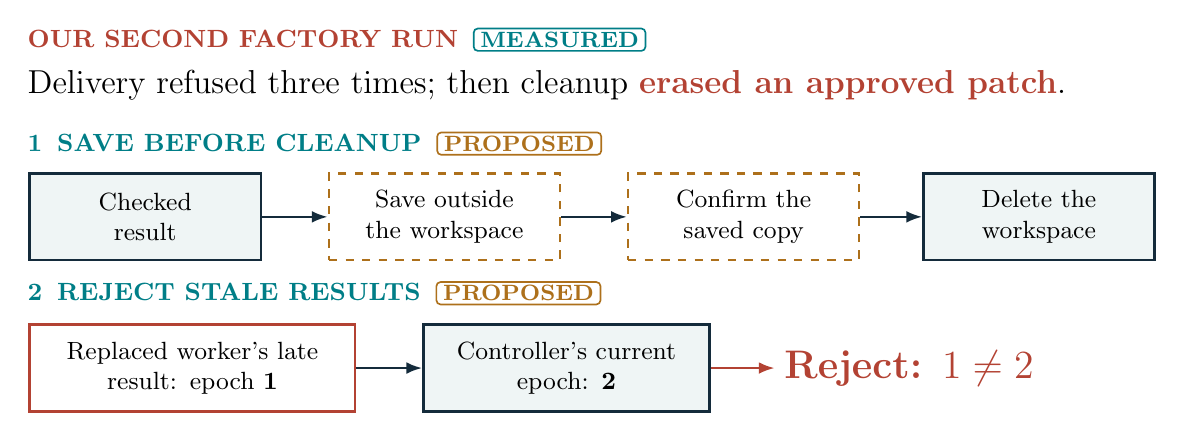
\begin{tikzpicture}[x=1cm,y=1cm,every node/.style={align=center,font=\fontsize{11.5}{14}\selectfont},
  head/.style={anchor=west,inner sep=0pt,font=\fontsize{9.5}{11}\selectfont\bfseries}]
\node[head,text=Rust] at (0,.8) {OUR SECOND FACTORY RUN\enspace\tagM};
\node[anchor=west,inner sep=0pt,font=\fontsize{12.5}{15}\selectfont] at (0,.22) {Delivery refused three times; then cleanup \textcolor{Rust}{\textbf{erased an approved patch}}.};
\node[head,text=Teal] at (0,-.52) {1\enspace SAVE BEFORE CLEANUP\enspace\tagP};
\node[state,text width=2.7cm,minimum height=1.1cm] (a) at (1.5,-1.45) {Checked\\result};
\node[proposed,text width=2.7cm,minimum height=1.1cm] (b) at (5.3,-1.45) {Save outside\\the workspace};
\node[proposed,text width=2.7cm,minimum height=1.1cm] (c) at (9.1,-1.45) {Confirm the\\saved copy};
\node[state,text width=2.7cm,minimum height=1.1cm] (d) at (12.85,-1.45) {Delete the\\workspace};
\draw[flow] (a)--(b);\draw[flow] (b)--(c);\draw[flow] (c)--(d);
\node[head,text=Teal] at (0,-2.42) {2\enspace REJECT STALE RESULTS\enspace\tagP};
\node[bad,text width=3.9cm,minimum height=1.1cm] (f) at (2.1,-3.37) {Replaced worker's late\\result: epoch \textbf{1}};
\node[state,text width=3.4cm,minimum height=1.1cm] (e) at (6.85,-3.37) {Controller's current\\epoch: \textbf{2}};
\node[text=Rust,font=\fontsize{14}{17}\selectfont\bfseries] (g) at (11.2,-3.37) {Reject: $1\ne2$};
\draw[flow] (f)--(e);\draw[denied] (e)--(g);
\end{tikzpicture}\end{center}
\claim{Proposed: an epoch fence, and a publish keyed by the digest.}
\sources{Second factory run: observed. Save order, epoch fence: proposed. Prior art: leases (1989), Chubby sequencers (2006).}
\qadetail{MEASURED scope: SELFHOST-3, from local run records that are not published; about 26 minutes wall time, 853.8 s of stage time, \$3.43, a reported suite count of 1,981 with no failures, and an approved review. Do not upgrade the reported count into a confirmed all-passed count. Delivery was refused three times with files outside the reviewed commit stream; the stray file was the harness's own review-diff archive mirrored into the workspace. Teardown removed the patch and no pull request resulted. It ran on Docker sandboxes, serially; nothing forked. This is a delivery and recovery incident, not a full second task reconstruction. DESIGN scope: the save, confirm, delete order is a proposed recovery rule; it was not executed in the incident, and export before cleanup is proposed, not merged. Confirming a saved copy requires retrievable exact artifact bytes and their evidence, not a hash alone. An approved review is distinct from a passed required behavioral check and from publication authorization; preserving refused candidates does not bypass the delivery gate. The epoch (a permission version number, a fencing token in the Chubby-sequencer sense) is a proposed publication protocol, not an implemented or model-checked result: a TLA+ design exists, with no TLC run or implementation trace check recorded. The controller checks authenticated identity, current epoch, expiry, artifact, scope and budget; evidence, approval and publication must name one frozen artifact. A fence rejects stale results; it does not by itself give exactly-once publication. Publish-once also needs an idempotent publish keyed by the artifact digest, so a controller crash between push and record cannot publish twice; if the controller is ever replicated, the repository itself must check the epoch. Replacement and concurrent fork are distinct: replacing logical worker w invalidates its old epoch, while a concurrent child gets a new worker identity and its own epoch and need not revoke a continuing parent. Fresh identity alone does not confer authority. Authorization is checked outside restored guest state, so a copied local generation value cannot establish current permission. Controller-held publication, with no publish key in the worker, was exercised in the factory runs. A replaced or restored worker may still try to deliver, which is why the fence lives in the controller. Prior art: leases (Gray and Cheriton, SOSP 1989); fencing tokens as in Chubby sequencers (Burrows, OSDI 2006).}
\note{[1:15] A checked result also has to survive. In a second factory run, review approved a patch, but delivery was refused three times over a stray file, the harness's own review archive. Then cleanup deleted the workspace and the approved patch. The fix is an order: save the result outside the workspace, confirm the copy, then delete. Saving is not permission to publish, and a replaced or restored worker may still try to deliver. So the controller keeps an epoch, a permission version number. Replacing a worker moves the epoch from one to two. A late result from the old worker still carries one, so the controller rejects it. Because the check lives in the controller, restoring a snapshot cannot revive an old permission. And a publish keyed by the digest makes a retry a no-op, like a cache hit. All proposed; the loss was real. What is still open?}
\end{frame}

\setact{6}
% Table helpers for this frame only: a gold rule row and a muted test cell with a status prefix.
\newcommand{\oqrule}[1]{\multicolumn{3}{@{}l}{\fontsize{9.5}{11}\selectfont\bfseries\color{Gold}#1}\\\midrule}
\newcommand{\oqtest}[2]{\leavevmode{\color{Muted}\textbf{#1:}\enspace#2}}
\begin{frame}[t]{\ev{\tagP}Five questions remain open; the preregistered tests have not started.}
\vspace{0pt}
{\fontsize{11}{13.5}\selectfont
\renewcommand{\arraystretch}{1.0}\begin{tabularx}{\linewidth}{@{}>{\bfseries\color{Teal}}l L{8.05cm}Y@{}}
\oqrule{COMPUTE ONCE}
1 & Does the snapshot we restore keep live memory? & \oqtest{Gate 0}{RAM-only nonce}\\
2 & Does restoring beat a warm cache? & \oqtest{H1}{N\,=\,3, 6, 12 sandboxes}\\[4pt]
\oqrule{COUNT ONCE}
3 & Do restored siblings fail together more? & \oqtest{H2}{race-test co-failure}\\
4 & When should the reducer refuse a precision claim? & \oqtest{Design}{dependence, calibration}\\[4pt]
\oqrule{PUBLISH ONCE}
5 & Does the epoch fence hold across restores? & \oqtest{Design}{TLA+, no TLC run}\\\bottomrule
\end{tabularx}\par}
\claim{Until Gate 0 runs: many restores of one snapshot, not a memory fork.}
\sources{PREREGISTRATION.md, tag prereg-v1 (amended to v3; no rule changed). Q5: TLA+ design, no TLC run.}

\qadetail{No result is claimed until the protocol runs. No decision rule has changed since prereg-v1 (later amendments de13c1d, prereg-v2 and prereg-v3 updated slide references and corrected a Phase B standard-error note); any change must be a dated amendment before collection. Gate 0 comes first, because H1's reached-state restore is only a disk restore if memory is not kept: a live process holds a random 128-bit nonce only in RAM; take a named snapshot, restore three children and check that the process is alive with the same nonce. It is a necessary probe, not a full fidelity proof; if the nonce does not survive, every report says restore fan-out. VM and process checkpoints (Xen save/restore, SnowFlock, Firecracker, CRIU) capture memory by design; the open question is whether the named-snapshot restore path we measured keeps it. Measured restore fan-out: a named 141 MB islo snapshot, restore--run--capture round trips, 255 of 256 succeeded at concurrency 12, p50 6.87 s, p95 9.04 s, client-measured, teardown excluded (arXiv:2607.09689v4, Table 2). These are API round trips, not mechanism latency or a provider ranking. H1: compare reached-state restore with a warm cached template at N = 3, 6 and 12 concurrent cells, 20 repetitions per arm and N, interleaved in random order; batch makespan is primary; gain is median cached minus median restore makespan, with 10,000 within-arm bootstrap resamples. It supports H1 if the 95\% lower confidence bound exceeds 10 s at every N and rejects if the Bonferroni 98.3\% upper bound is below 10 s at any N; other outcomes are inconclusive. Cold start is a reference only. Capture accounting and resource cost are not makespan. H2: 12 snapshot families of 3 restored siblings; strangers are restores from other families started in the same slot, so both arms restore and only shared ancestry differs. The statistic is the intraclass correlation of race-test outcomes; support needs a one-sided permutation p below 0.05 and an excess above 0.05, and rejection (90\% upper bound below 0.05) rules out a shared-ancestry excess of 0.05 or more, not all dependence. H2 measures environmental race-test co-failure, not dependence between agent judgments. Reused families and repeated rounds make pair differences dependent; an analysis amendment is proposed and must precede collection. Reducer: the built reducer rejects repeated declared evidence IDs and carries lineage; abstention when dependence is unknown and a controller-derived precision are proposed. Distinct IDs do not prove independence. Question 5: the epoch fence and promotion rule exist as a TLA+ design model with no TLC run or trace check recorded, so neither has been model-checked; restores and controller crashes are the cases to check. Beyond the five, the companion note (Speculative Sandboxes, 13 Oct 2026) asks when a fork should exist at all: it writes the probability that any branch is accepted with the chain rule over earlier failures, which does not assume independent siblings; its Python controller is a finite-world mock, not a forked islo integration. Acceptance and correctness are different variables.}
\note{[1:10] Five questions remain open. Three have preregistered tests; none has started. Compute once. First, does the snapshot we restore keep live memory? VM and process checkpoints can; we have not shown that ours does. A nonce held only in RAM must survive into three restored children. Until then, I say restore fan-out, not memory fork. Second, does restoring beat a warm cache, at three, six and twelve parallel sandboxes? Count once. Third, do restored siblings fail a race test together more than restores of other snapshots? That measures shared-environment failures, not whether agents' judgments are independent. Fourth, a design question: when should the reducer refuse a precision claim? Publish once. Fifth: does the epoch fence hold across restores? We have a TLA+ model, not yet model-checked. A companion note asks when a fork should exist at all. Now, the contributions.}
\end{frame}

\setact{7}
% THE MAP, third of three uses (03, 15, 26). The \providecommand block below is copied verbatim from 03-promise.tex; keep the three identical.
% Arguments: #1 #2 #3 = column bodies (compute once, count once, publish once); #4 = extra TikZ.
\providecommand{\rulemap}[4]{%
\noindent\begin{tikzpicture}[x=1cm,y=1cm,
  rh/.style={evidence,text width=4.2cm,minimum height=.9cm,font=\fontsize{12}{14}\selectfont\bfseries,text=Teal},
  rs/.style={anchor=north,inner sep=0pt,font=\fontsize{10}{12}\selectfont,text=Muted},
  rb/.style={anchor=north,inner sep=0pt,text width=4.7cm,align=center,font=\fontsize{12}{14.5}\selectfont}]
\useasboundingbox (0,1.05) rectangle (14.4,-3.75);
\node[rh] (r1) at (2.3,0) {1\enspace COMPUTE ONCE};
\node[rh] (r2) at (7.2,0) {2\enspace COUNT ONCE};
\node[rh] (r3) at (12.1,0) {3\enspace PUBLISH ONCE};
\draw[flow] (r1)--(r2);\draw[flow] (r2)--(r3);
\draw[message] (r3.north)--++(0,.42)-|node[pos=.25,above,inner sep=1.5pt,font=\fontsize{9}{10}\selectfont,text=Teal]{continue} (r1.north);
\node[rs] at (2.3,-.62) {Runtime};
\node[rs] at (7.2,-.62) {Evidence};
\node[rs] at (12.1,-.62) {Acceptance};
\node[rb] at (2.3,-1.15) {#1};
\node[rb] at (7.2,-1.15) {#2};
\node[rb] at (12.1,-1.15) {#3};
#4
\end{tikzpicture}\par}
\begin{frame}[t]{\ev{\tagB\,\tagP}\surf{THREE RULES}Contributions: three rules for doing work once.}
\vspace{.1cm}
\rulemap{\fontsize{11}{12.5}\selectfont\textbf{A cost rule}\\[2pt]{\color{Gold}\mbox{$(N{-}1)P > H+N(R{+}D)$}}\\[2pt]{\color{Gold}against a warm cache}\par}
{\fontsize{11}{12.5}\selectfont\textbf{An evidence contract}\\[2pt]Duplicate IDs rejected\\[2pt]{\color{Gold}Receipts outside the child}\\[2pt]{\color{Gold}Shared errors weighted}\par}
{\fontsize{11}{12.5}\selectfont\textbf{An acceptance gate}\\[2pt]Exact bytes, controller key\\[2pt]{\color{Gold}A test per promise}\\[2pt]{\color{Gold}Epoch fence}\par}
{\foreach \xx/\lab/\nn in {2.3/a hash keys the cache/h1,7.2/binds the receipt/h2,12.1/names the published bytes/h3}{\node[inner xsep=3pt,inner ysep=1pt,font=\fontsize{10.5}{12.5}\selectfont,text=Teal] (\nn) at (\xx,-3.5) {\lab};}
\draw[Teal,densely dashed,line width=.8pt,-{Latex[length=1.6mm]}] (h1)--(h2);\draw[Teal,densely dashed,line width=.8pt,-{Latex[length=1.6mm]}] (h2)--(h3);}
\claim{\centering\forktree\enspace Compute once. Count once. Publish once.}
\sources{Built: publish check, duplicate-ID reducer. Measured: serial factory runs, nothing forked. Gold: proposed or modelled.}
\qadetail{The map from slide 3 a third time: each question now has its contribution. The contribution claim is the integrated execution, evidence and acceptance contract; forking, caching, testing, review and provenance are established techniques, and no claim of invention, comprehensive priority or measured parallel speedup is made. Status by part: the cost rule is an additive resource model, priced against the warm alternative (restoring saved state versus rebuilding with a warm cache, both forms of reuse); H1 compares restoring a reached state with a warm cached template at N = 3, 6, 12 with batch makespan as the primary endpoint, which is not the same as total resource cost, and it has not started. The built reducer rejects duplicate declared observation IDs and carries lineage, but it does not abstain on dependence, and distinct IDs do not prove independence; typed receipts written outside the child and covariance weighting of shared errors are proposed. The factory runs exercised controller-held publication with no publish key in the worker, serially on Docker sandboxes, with nothing forked; the sha256-bound publish check is built; a required test for each promise, an external evaluator and the epoch fence are proposed (a TLA+ design exists, with no TLC run). A hash proves identity, not correctness. Two research questions remain: can an ancestry, fixtures and feedback manifest support a calibrated dependence model or a justified refusal of a precision claim, and can restore renew authority and reject stale publication across failure and uncertain external effects?}
\note{[1:00] My contributions, on the same map we started with. Compute once: a cost rule. Restore saved state only when the setup it avoids exceeds the overhead it adds, priced against a warm cache. Count once: an evidence contract. The reducer I built rejects duplicate observation IDs; receipts kept outside the child and weighting of shared errors are proposed. Publish once: an acceptance gate. The controller holds the key and publishes exact bytes; that check is built. A test for every promise and the epoch fence are proposed. One hash threads all three: it keys the cache, binds the receipt, and names the published bytes. It proves identity, not correctness. Compute once. Count once. Publish once. Your questions, please.}
\end{frame}

\end{document}
